\chapter[Статические и динамические матрицы]{Статические и динамические матрицы}\label{ch06}
Данная глава посвящена обработке матриц в \Sys{С++}, на большом количестве примеров будут рассмотрены возможности языка для
обработки статических и динамических матриц. В завершающем параграфе будут рассмотрено использование двойных указателей
и функций на примере решения задач линейной алгебры.

\section[Статические матрицы \Sys{С(С++)}]{Статические матрицы \Sys{С(С++)}}
Матрица --- это двумерный массив, каждый элемент которого имеет два индекса: номер строки --- $i$; номер столбца --- $j$. 

Статический двумерный массив (матрицу) можно объявить так:

\Sys{тип имя\_переменной [n][m];}

где тип определяет тип элементов массива, \Sys{имя\_переменной} --- имя матрицы, $n$ --- количество строк, $m$ --- количество столбцов в матрице. Строки нумеруются от 0 до $n-1$, столбцы --- от 0 до $m-1$.

Например, 

\Sys{double x[20][35];}

Описана матрица вещественных чисел $x$, состоящая из 20 строк и 35 столбцов 
(строки нумеруются от 0 до 19, столбцы от 0 до 34).

Как и любой другой переменной, матрице можно присвоить начальное значение, например 
\Sys{int A[2][3]=\{\{1,2,3\}, \{4,5,6\}\};}

Для обращения к элементу матрицы необходимо указать ее имя, и в квадратных скобках номер строки, а затем в квадратных
скобках --- номер столбца. Например, \Sys{x[2][4]} --- элемент матрицы $x$, находящийся в третьей строке и пятом
столбце\footnote{Напоминаем, что нумерация строк и столбцов идет с 0.}.

Для работы с элементами матрицы необходимо использовать два цикла. Для построчной обработки матрицы значениями параметра
первого (внешнего) цикла будут номера строк матрицы, значениями параметра второго (внутреннего) цикла --- номера столбцов
(см. рис.~\ref{ch06:refDrawing0}). При построчной обработке матрицы вначале поочерёдно рассматриваются элементы первой
строки (столбца), затем второй и т.д. до последней. Если необходимо обрабатывать матрицу по столбцам, то необходимо
организовать внешний цикл по столбцам, а внутренний по строкам (см.~рис.~\ref{ch06:refDrawing1}).

\section{Динамические матрицы}
В предыдущем параграфе мы рассмотрели описание статических матриц, в этом случае память для хранения матрицы выделяется
в момент описания. Однако в \Sys{С++} существует возможность создавать динамические матриц. Динамические матрицы
можно создавать с использованием обычных указателей и с помощью двойных указателей. Рассмотрим оба способа работы с
динамическими матрицами последовательно. 

%%%% рис 6.1 и 6.2 бок о бок
\begin{figure}[H]
\begin{floatrow}
\floatbox{figure}[.45\textwidth][\FBheight][t]
{\caption{Блок-схема построчной обработки матрицы}
\label{ch06:refDrawing0}}
{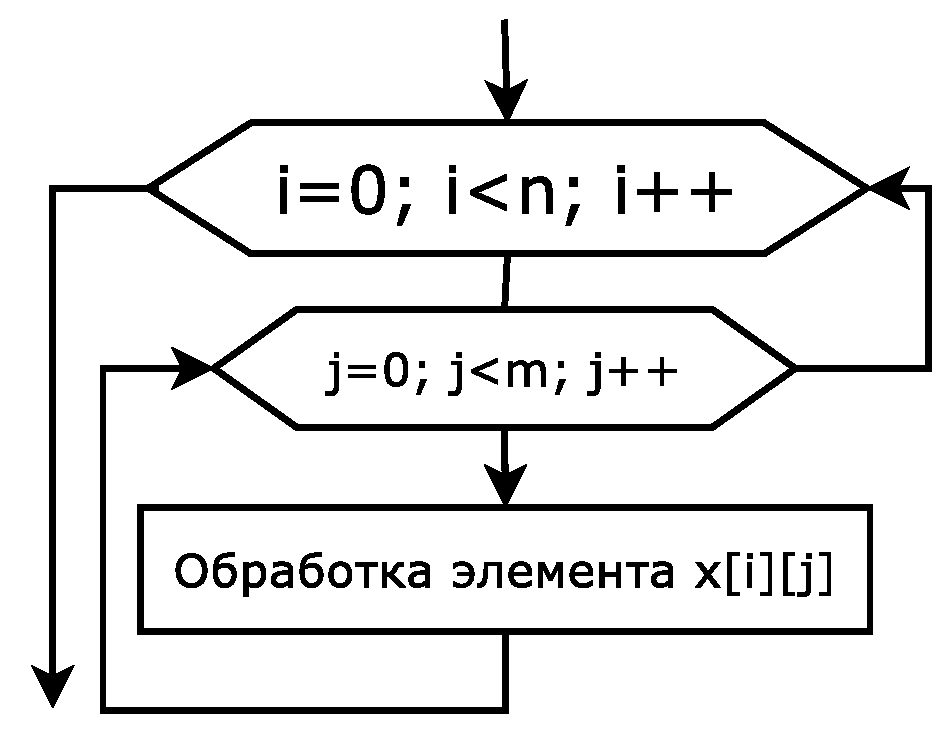
\includegraphics[width=0.45\textwidth,keepaspectratio]{img/ris_6_1}}\hspace*{0.05\textwidth}
%
\floatbox{figure}[.45\textwidth][\FBheight][b]
{\caption{Блок-схема обработки матрицы по столбцам}
\label{ch06:refDrawing1}}
{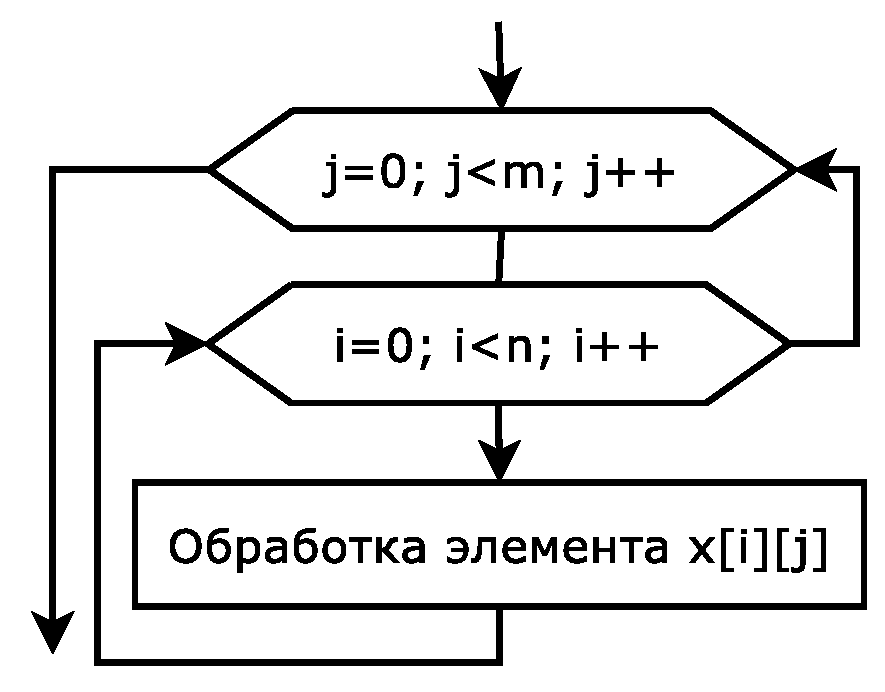
\includegraphics[width=0.45\textwidth,keepaspectratio]{img/ris_6_2}}
\end{floatrow}
\end{figure}


\subsection[Использование указателей для работы с динамическими матрицами]{Использование указателей для работы с
динамическими матрицами}
При работе с динамическими матрицами можно использовать обычные указатели. После описания указателя, необходимо будет
выделить память для хранения $N\times M$ элементов ($N$ --- число строк, $M$ --- число столбцов). Рассмотрим
в качестве примера выделение памяти для хранения целочисленной матрицы размером $N\times M$.
\begin{lstlisting}
int *A, n, m;
A=(int *) calloc (N*M, sizeof(int));
\end{lstlisting}
Для выделения памяти можно использовать также и функцию \Sys{malloc} 
\begin{lstlisting}
A=(int *) malloc (N*M*sizeof(int));
\end{lstlisting}
или операцию \Sys{new}
\begin{lstlisting}
A=new int [N*M];
\end{lstlisting}

Память мы выделили, осталось найти способ обратиться к элементу матрицы. Все элементы матрицы хранятся в одномерном
массиве размером $N\times M$ элементов. Сначала в этом массиве расположена 0-я строка матрицы, затем 1-я и т.д.
Поэтому для обращения к элементу \Sys{A[i][j]} необходимо, по номеру строки $i$ и номеру столбца $j$ вычислить номер этого
элемента $k$ в динамическом массиве. Учитывая, что в массиве элементы нумеруются с нуля
$k=iM+j$. Обращение к элементу \Sys{A[i][j]}
будет таким \Sys{*(A+i*m+j)}.

\subsection[Использование двойных указателей для работы с динамическими матрицами]{Использование двойных указателей
для работы с динамическими матрицами}
Основной способ работы с динамическими матрицами базируется на использовании двойных указателей. Рассмотрим следующий
фрагмент программы.
\begin{lstlisting}
int main()
{
  int N,M; 
  float **a;
  a=new float *[N];
}
\end{lstlisting}

С помощью оператора \Sys{new} создан массив из $n$ элементов\footnote{В данном случае массив указателей 
на \Sys{float}.}, в котором
каждый элемент является адресом, где хранится указатель (фактически каждый указатель --- адрес строки матрицы). Осталось
определить значение элементов массива. Для этого организуем цикл (переменная цикла $i$ изменяется от 0 до
$N-1$), в котором будет выделяться память для хранения очередной строки матрицы. Адрес этой строки будет
записываться в \Sys{a[i]}.
\begin{lstlisting}
for(i=0;i<N;i++)
a[i]=new float(M);
\end{lstlisting}

После этого определён массив $N$ указателей, каждый из которых адресует массив из $M$ чисел (в данном
случае вещественных типа \Sys{float}). Фактически создана динамическая матрица размера $N\times M$.
Обращение к элементу
динамической матрицы идет так же, как и к элементу статической матрицы. Для того, чтобы обратиться к элементу 
$a_{i,j}$ в программе на \Sys{C++} необходимо указать ее имя, и в квадратных скобках номер строки 
и столбца (\Sys{a[i][j]}).

\section[Обработка матриц в \Sys{С(С++)}]{Обработка матриц в \Sys{С(С++)}}
Рассмотрим основные операции, выполняемые над матрицами (статическими и динамическими) при решении задач.

Матрицы, как и массивы, нужно вводить (выводить) поэлементно. Блок-схема ввода элементов матрицы \Sys{x[n][m]} изображена на
рис.~\ref{ch06:refDrawing2}.

%%%% рис 6.3 и 6.4 бок о бок
\begin{figure}[H]
\begin{floatrow}
\floatbox{figure}[.35\textwidth][\FBheight][t]
{\caption{Ввод элементов матрицы}
\label{ch06:refDrawing2}}
{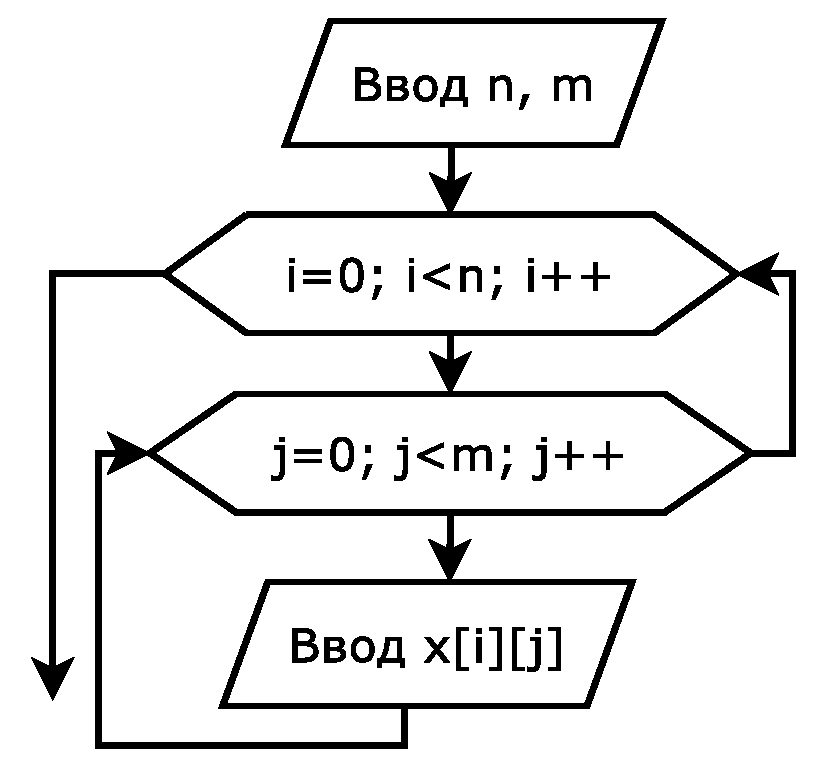
\includegraphics[width=0.45\textwidth,keepaspectratio]{img/ris_6_3}}\hspace*{0.05\textwidth}
%
\floatbox{figure}[.55\textwidth][\FBheight][b]
{\caption{Блок-схема построчного вывода матрицы}
\label{ch06:refDrawing3}}
{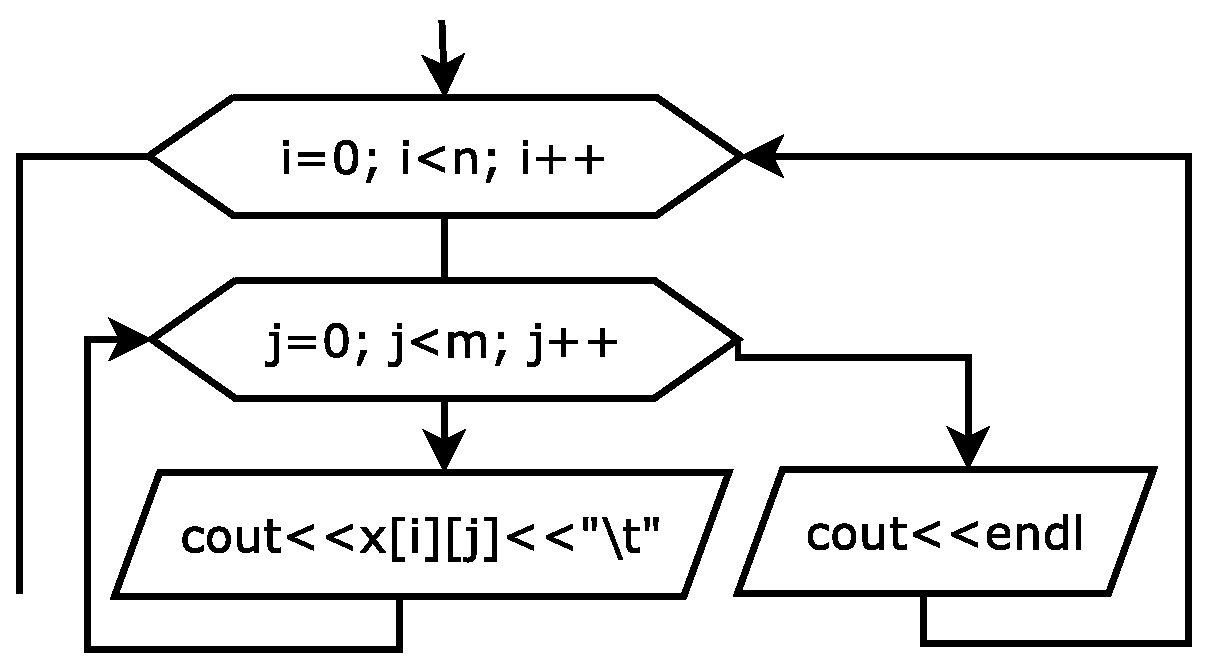
\includegraphics[width=0.45\textwidth,keepaspectratio]{img/ris_6_4}}
\end{floatrow}
\end{figure}


При выводе матрицы элементы располагаются построчно, например:
$$\begin{matrix}6&-9&7&13\\5&8&3&8\\3&7&88&33\\55&77&88&37\end{matrix}$$

Алгоритм построчного вывода элементов матрицы приведен на рис.~\ref{ch06:refDrawing3}.


Ниже приведен текст программы на \Sys{C++} ввода-вывода статической матрицы.
\begin{lstlisting}
#include <iostream>
using namespace std;
int main()
{
  int i,j,N,M,a[20][20];
  cout<<"N=";
//`Ввод количества строк`
  cin>>N;
  cout<<"M=";
//`Ввод количества столбцов`
  cin>>M;
  cout<<"`Ввод матрицы` A"<<endl;
//`Цикл по переменной` i, `в котором перебираем строки матрицы`
  for(i=0;i<N;i++)
//`Цикл по переменной` j, `в котором перебираем элементы внутри строки`
    for(j=0;j<M;j++)
//`Ввод очередного элемента матрицы`
      cin>>a[i][j];
  cout<<"`Вывод матрицы` A"<<endl;
//`Цикл по переменной` i, `в котором перебираем строки матрицы`
  for(i=0;i<N;i++)
  {
//`Цикл по переменной` j, `в котором перебираем строки матрицы`
    for(j=0;j<M;j++)
//`Вывод очередного элемента матрицы`
      cout<<a[i][j]<<"\t";
//`По окончанию вывода всех элементов строки --- переход на новую строку.`
    cout<<endl;
  }
}
\end{lstlisting}

Цикл для построчного вывода матрицы можно записать и так.
\begin{lstlisting}
for(i=0;i<N;cout<<endl,i++)
  for(j=0;j<M;j++)
    cout<<a[i][j]<<"\t";
\end{lstlisting}
При вводе матрицы элементы каждой строки можно разделять пробелами, символами табуляции или
\Sys{Enter}\footnote{Элементы каждой строки можно разделять пробелами или символами табуляции, а в конце
строки нажимать \Sys{Enter}.}. 
%На рис.~\ref{ch06:refDrawing4} 
Ниже 
представлены результаты работы программы.
\begin{verbatim}
N=4
M=5
Ввод матрицы A
1 2 3
5 4
3 6 7 8 9
1 2 3 4 5 6 7 8 9 0
Вывод матрицы A
1       2       3       5       4	
3       6       7       8       9	
1       2       3       4       5	
6       7       8       9       0
\end{verbatim}

Далее на примерах решения практических задач будут рассмотрены основные алгоритмы обработки матриц и их реализация в
\Sys{C++}. Перед этим, давайте, вспомним некоторые свойства матриц (рис.~\ref{ch06:refDrawing5}):

\begin{itemize}
\item если номер строки элемента совпадает с номером столбца ($i=j$), это означает что элемент лежит на главной
диагонали матрицы; 
\item если номер строки превышает номер столбца ($i>j$), то элемент находится ниже главной диагонали;
\item если номер столбца больше номера строки ($i<j$), то элемент находится выше главной диагонали.
\item элемент лежит на побочной диагонали, если его индексы удовлетворяют равенству  $i+j=n-1$ ; 
\item неравенство  $i+j<n-1$  характерно для элемента находящегося выше побочной диагонали;
\item соответственно, элементу лежащему ниже побочной диагонали соответствует выражение  $i+j>n-1$.
\end{itemize}


\begin{figure}[htb]
\begin{center}
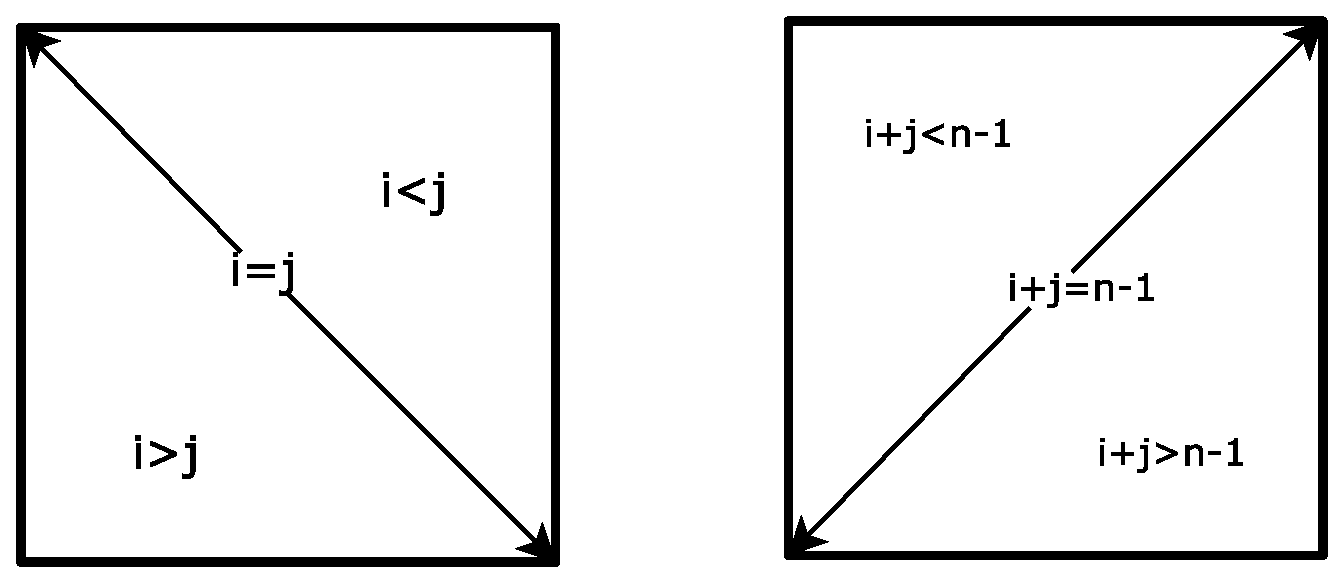
\includegraphics[width=0.7\textwidth]{img/ris_6_6}
\caption{Свойства элементов матрицы}
\label{ch06:refDrawing5}
\end{center}
\end{figure}

\prg{Найти сумму элементов матрицы, лежащих выше главной
диагонали.}{gl06:prg0}

Алгоритм решения данной задачи (рис.~\ref{ch06:refDrawing6}) построен следующим образом: обнуляется ячейка для
накапливания суммы (переменная $s$). Затем с помощью двух циклов (первый по строкам, второй по столбцам) просматривается
каждый элемент матрицы, но суммирование происходит только в том случае если, этот элемент находится выше главной
диагонали (при выполнении условия  $i<j$).

%\begin{figure}[htb]
%\begin{center}
%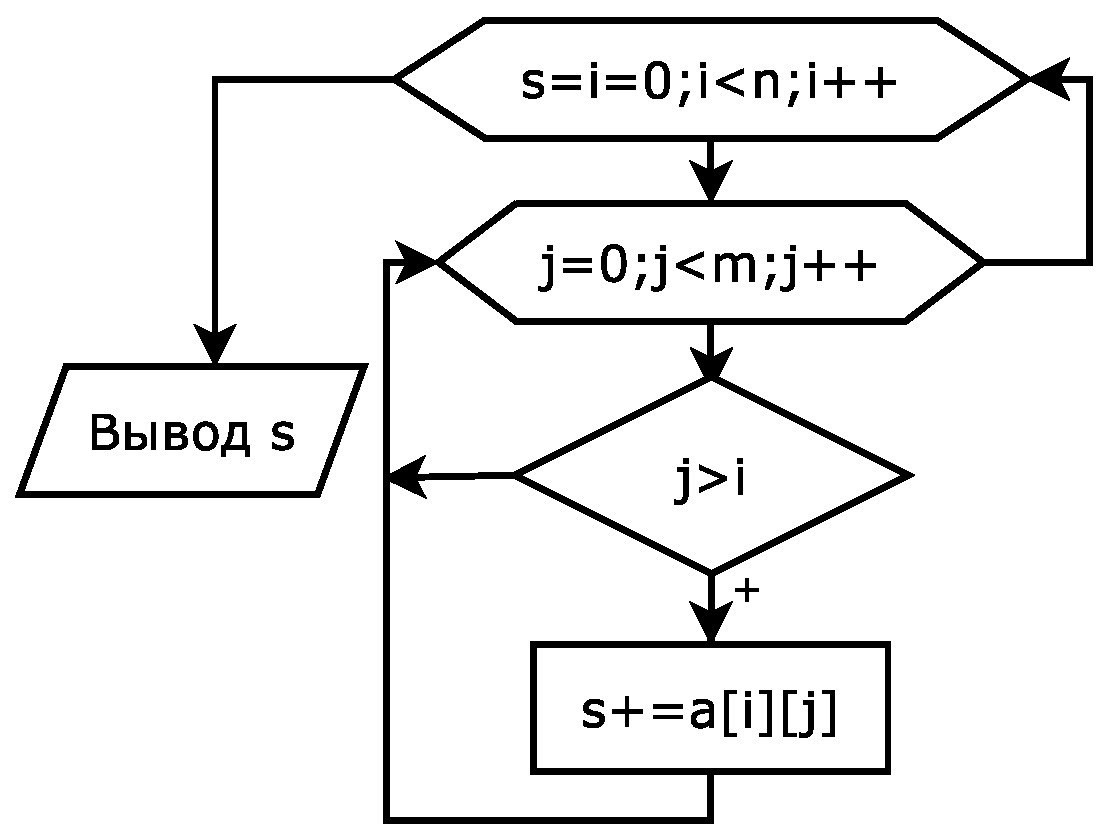
\includegraphics[width=0.5\textwidth]{img/ris_6_7}
%\caption{Блок-схема задачи \ref{gl06:prg0} (алгоритм 1).}
%\label{ch06:refDrawing6}
%\end{center}
%\end{figure}

%%%% рис 6.7 и 6.8 бок о бок
\begin{figure}[H]
\begin{floatrow}
\floatbox{figure}[.45\textwidth][\FBheight][t]
{\caption{Блок-схема задачи \ref{gl06:prg0} (алгоритм 1).}
\label{ch06:refDrawing6}}
{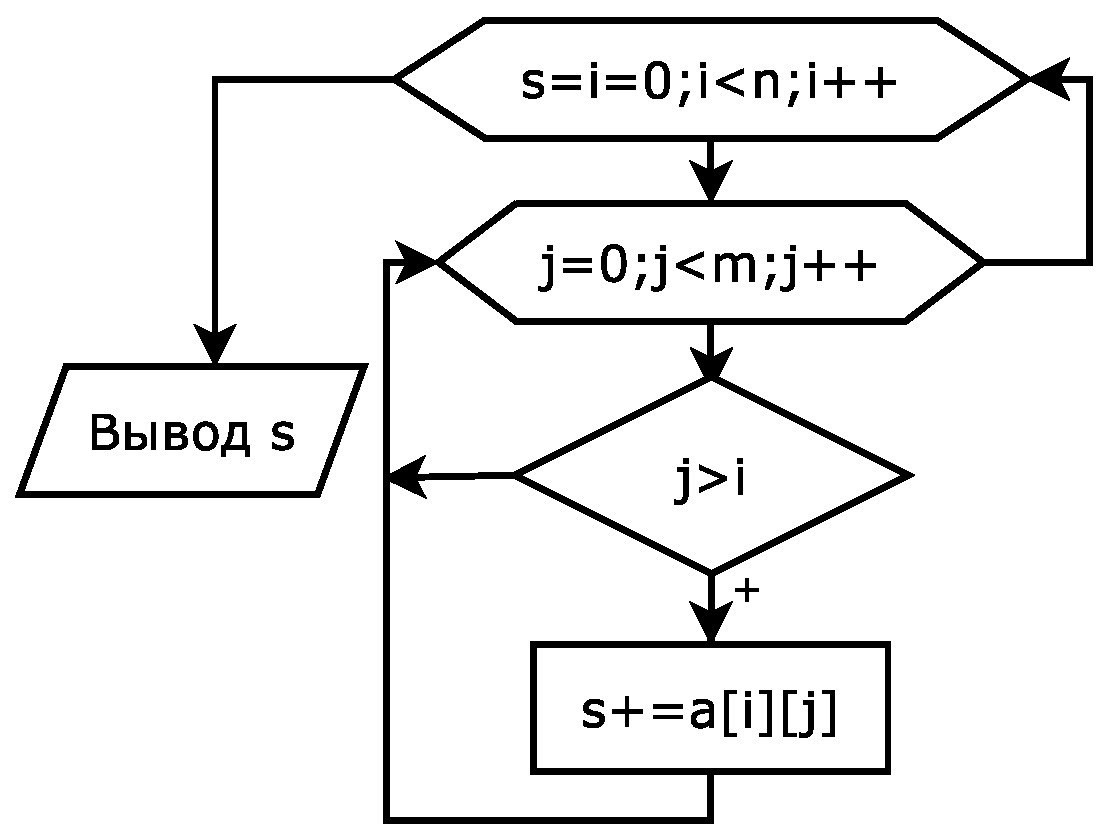
\includegraphics[width=0.45\textwidth,keepaspectratio]{img/ris_6_7}}\hspace*{0.05\textwidth}
%
\floatbox{figure}[.45\textwidth][\FBheight][b]
{\caption{Блок-схема задачи \ref{gl06:prg0} (алгоритм 2).}
\label{ch06:refDrawing7}}
{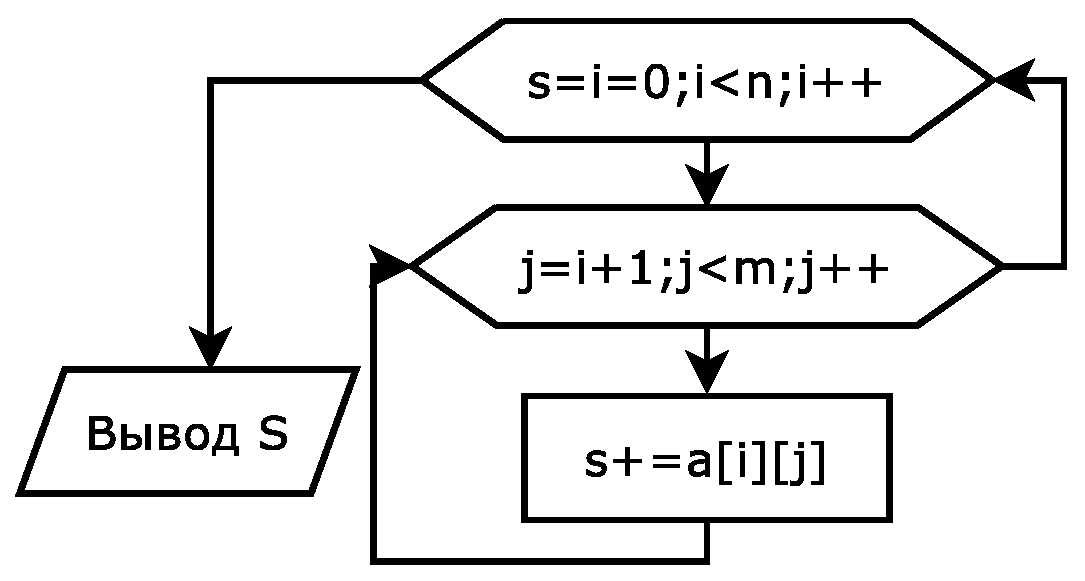
\includegraphics[width=0.45\textwidth,keepaspectratio]{img/ris_6_8}}
\end{floatrow}
\end{figure}



Текст программы: 
\begin{lstlisting}
#include <iostream>
using namespace std;
int main()
{
  int s,i,j,n,m,a[20][20]; 
  cout<<"N=";
  cin>>n;
  cout<<"M=";
  cin>>m;
  cout<<"`Ввод матрицы` A"<<endl;
  for(i=0;i<n;i++)
    for(j=0;j<m;j++)
      cin>>a[i][j];
  for(s=i=0;i<n;i++)
    for(j=0;j<m;j++)
//`Если элемент лежит выше главной диагонали, то наращиваем сумму.` 
      if (j>i) s+=a[i][j];
  cout<<"S="<<s<<endl;
}
\end{lstlisting}

На рис.~\ref{ch06:refDrawing7} изображён ещё один вариант решения данной задачи. 
В нем проверка условия  $i<j$ не выполняется, но, тем не менее, в нем так же 
суммируются элементы матрицы, находящиеся выше главной диагонали. В
нулевой строке заданной матрицы необходимо сложить все элементы, начиная с первого. Во первой --- все, начиная со
второго, в $i$–й строке процесс начнётся с $(i+1)$–го элемента и так далее. Таким образом, внешний цикл работает от 0 до
$N-1$, а второй от $i+1$ до $M$. Авторы надеются, что читатель самостоятельно составит программу, соответствующую
описанному алгоритму.

%\begin{figure}[htb]
%\begin{center}
%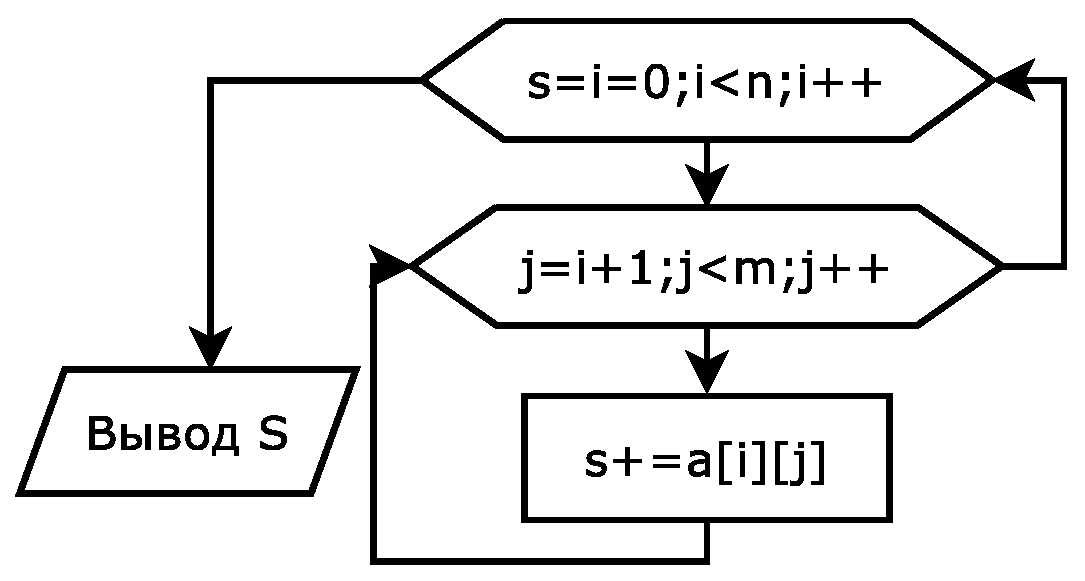
\includegraphics[width=0.5\textwidth]{img/ris_6_8}
%\caption{Блок-схема задачи \ref{gl06:prg0} (алгоритм 2).}
%\label{ch06:refDrawing7}
%\end{center}
%\end{figure}

\prg{Вычислить количество положительных элементов квадратной
матрицы, расположенных по ее периметру и на диагоналях. Напомним, что в квадратной матрице число строк равно числу
столбцов.}{gl06:prg1} 

Прежде чем приступить к решению задачи рассмотрим рисунок~\ref{ch06:refDrawing8}, на котором изображена схема квадратных
матриц различной размерности. 

\begin{figure}[htb]
\begin{center}
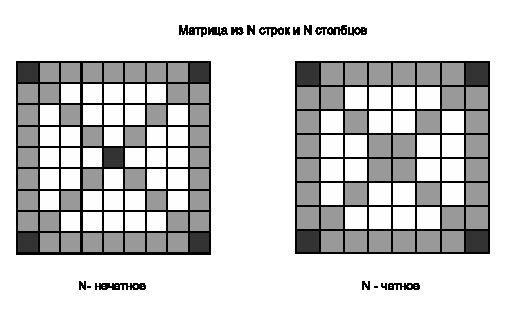
\includegraphics[width=0.7\textwidth]{img/ris_6_9}
\caption{Рисунок к задаче~\ref{gl06:prg1}.}
\label{ch06:refDrawing8}
\end{center}
\end{figure}

Из условия задачи понятно, что не нужно рассматривать все элементы заданной матрицы. Достаточно просмотреть первую и
последнюю строки, первый и последний столбцы, а так же диагонали. Все эти элементы отмечены на схеме, причём чёрным
цветом выделены элементы, обращение к которым может произойти дважды. Например, элемент с номером $(0,0)$ принадлежит как
к нулевой строке, так и к нулевому столбцу, а элемент с номером $(N-1,N-1)$
находится в последней строке и последнем столбце одновременно. Кроме того, если $N$ --- число нечётное 
(на рисунке~\ref{ch06:refDrawing8} эта матрица расположена слева), то существует элемент с номером $(N/2, N/2)$,
который находится на пересечении главной и побочной диагоналей. При нечётном значении $N$ (матрица справа на
рис.~\ref{ch06:refDrawing8}) диагонали не пересекаются.

Итак, разобрав подробно постановку задачи, рассмотрим алгоритм ее решения. Для обращения к элементам главной диагонали
вспомним, что номера строк этих элементов всегда равны номерам столбцов. Поэтому, если параметр $i$ изменяется
циклически от 0 до $N-1$, то \Sys{A[i][i]} --- элемент главной диагонали. Воспользовавшись
свойством, характерным для элементов побочной диагонали получим:

$i+j+1=N \longrightarrow j=N-i-1$,\\
следовательно, для $i=0,1,\dots,N-1$ элемент \Sys{А[i][N-i-1]} ---
элемент побочной диагонали. Элементы, находящиеся по периметру матрицы записываются 
следующим образом: \Sys{А[0][i]}
--- нулевая строка, \Sys{А[N-1][i]} --- последняя строка и соответственно \Sys{А[i][0]} --- нулевой столбец,
\Sys{А[i][N-1]} --- последний столбец.

Текст программы решения задачи с пояснениями приведён далее.
\begin{lstlisting}
#include <iostream>
using namespace std;
int main()
{
  int k,i,j,N,a[20][20]; 
  cout<<"N=";
  cin>>N;
  cout<<"`\Sys{Ввод матрицы}` A"<<endl;
  for(i=0;i<N;i++)
    for(j=0;j<N;j++)
      cin>>a[i][j];
//k` --- количество положительных элементов матрицы,` 
//`расположенных по ее периметру и на диагоналях.`
  for(i=k=0;i<N;i++)
  {
//`Элемент лежит на главной диагонали.`
    if(a[i][i]>0)k++;
//`Элемент лежит на побочной диагонали.`
    if(a[i][N-i-1]>0)k++;
  }
  for(i=1;i<N-1;i++)
  {
//`Элемент находится в нулевой строке.`
    if(a[0][i]>0)k++;
//`Элемент находится в последней строке.`
    if(a[N-1][i]>0)k++;
//`Элемент находится в нулевом столбце.`
    if(a[i][0]>0)k++;
//`Элемент находится в последнем столбце.`
    if(a[i][N-1]>0)k++;
  }
//`Если элемент, находящийся на пересечении диагоналей подсчитан дважды,`
//`то уменьшить вычисленное значение к на один.` 
  if ((N%2!=0)&&(a[N/2][N/2]>0))k--;
  cout<<"k="<<k<<endl;
}
\end{lstlisting}


\prg{Проверить, является ли заданная квадратная матрица единичной.}{gl06:prg2}

Единичной называют матрицу, у которой элементы главной диагонали --- единицы, а все остальные --- нули. Например, 
$$\left(\begin{matrix}1&0&0&0&0\\0&1&0&0&0\\0&0&1&0&0\\0&0&0&1&0\\0&0&0&0&1\end{matrix}\right)$$

Решать задачу будем так. Предположим, что матрица единичная и попытаемся доказать обратное. Если окажется, что хотя бы
один диагональный элемент не равен единице, или любой из элементов вне диагонали не равен нулю, то матрица единичной не
является. Воспользовавшись логическими операциями языка \Sys{С(С++)} все эти условия можно соединить в одно и составить программу,
текст которой приведён ниже.
\begin{lstlisting}
#include <iostream>
using namespace std;
int main()
{
  int pr,i,j,N, **a; 
//`Ввод размерности матрицы`
  cout<<"N=";
  cin>>N;
//`Создаём квадратную динамическую матрицу`
  a=new int *[N];
  for(i=0;i<N;i++)
    a[i]=new int [N];
  cout<<"`\Sys{Ввод элементов матрицы}` A"<<endl;
  for(i=0;i<N;i++)
    for(j=0;j<N;j++)
      cin>>a[i][j];
//`Предположим, что матрица единичная и присвоим переменной pr значение 1` 
//`(истина). Если значение этой переменной при выходе из цикла не изменится,` 
//`это будет означать, что матрица действительно единичная.`
  for(pr=1,i=0;i<N;i++)
    for(j=0;j<N;j++)
      if (((i==j)&&(a[i][j]!=1))||((i!=j)&&(a[i][j]!=0)))
//`Если элемент лежит на главной диагонали и не равен`
//`единице или элемент лежит вне главной диагонали и не равен нулю, то` 
      {
//`Переменной pr присвоить значение 0 (ложь), это будет означать,` 
//`что матрица единичной не является, и выйти из цикла.`
        pr=0;
        break;
      }
//`Проверка значения переменной pr и вывод соответствующего сообщения.` 
  if (pr) cout<<"`Единичная матрица`\n";
  else cout<<"`Матрица не является единичной`\n";
}
\end{lstlisting}

\prg{Преобразовать исходную матрицу так, чтобы нулевой элемент каждой строки был
заменён средним арифметическим элементов этой строки.}{gl06:prg3}

Для решения данной задачи необходимо найти в каждой строке сумму элементов, которую разделить на их количество.
Полученный результат записать в нулевой элемент соответствующей строки. Текст программы приведён далее.
\begin{lstlisting}
#include <iostream>
using namespace std;
int main()
{
  int i,j,N,M;
  double S, **a;
//`Ввод размерности матрицы.`
  cout<<"N=";
  cin>>N;
  cout<<"M=";
  cin>>M;
//`Создаём динамическую матрицу`
  a=new double *[N];
  for(i=0;i<N;i++)
    a[i]=new double [M];
  cout<<"`\Sys{Ввод элементов матрицы}` A"<<endl;
  for(i=0;i<N;i++)
    for(j=0;j<M;j++)
      cin>>a[i][j];
//`Цикл по `i` завершается записью среднего значения в`
//`нулевой элемент строки и наращиванием `i.
  for(i=0;i<N;a[i][0]=S/M,i++)
//`Вычисление суммы элементов строки.`
    for(S=j=0;j<M;j++)
      S+=a[i][j];
  cout<<"`\Sys{Преобразованная матрица}` A"<<endl;
  for(i=0;i<N;cout<<endl,i++)
    for(j=0;j<M;j++)
      cout<<a[i][j]<<"\t";
}
\end{lstlisting}

\prg{Задана матрица $A(n,m)$.
Поменять местами её максимальный и минимальный элементы.}{gl06:prg4}

Алгоритм решения этой задачи следующий: находим максимальный элемент матрицы \Sys{(max)} и его индексы
\Sys{(imax, jmax),} а также минимальный \Sys{(min)} и его индексы \Sys{(imin, jmin)}. После
чего элементы \Sys{A[imax][jmax]} и \Sys{A[imin][jmin]} поменяем местами. Для поиска максимального 
элемента и его индексов в
переменную \Sys{max} запишем \Sys{A[0][0]}, в переменные \Sys{imax}, \Sys{jmax}, (номер
строки и столбца, где находятся максимальный элемент) запишем 0. Затем в двойном цикле 
(цикл по переменной $i$ ---
по строкам, цикл по переменной $j$ --- по столбцам) перебираем все элементы, и каждый из них сравниваем с
максимальным (со значением переменной \Sys{max}). Если текущий элемент массива оказывается больше
максимального, то его переписываем в переменную \Sys{max}, а в переменную \Sys{imax} --- текущее
значение индекса $i$, в переменную \Sys{jmax} --- текущее значение $j$. Поиск минимального элемента
матрицы аналогичен, и отличается только знаком операции сравнения. Далее представлен текст программы решения задачи~\ref{gl06:prg4}.
\begin{lstlisting}
#include <iostream>
using namespace std;
int main()
{
int i,j,imax,jmax,imin,jmin,N,M;
double min,max,b, **a; 
//`Ввод размеров матрицы.` 
cout<<"N=";
cin>>N;
cout<<"M=";
cin>>M;
//`Создаём динамическую матрицу`
a=new double *[N];
for(i=0;i<N;i++)
  a[i]=new double [M];
cout<<"`\Sys{Ввод элементов матрицы}` A"<<endl;
for(i=0;i<N;i++)
  for(j=0;j<M;j++)
    cin>>a[i][j];
//`Двойной цикл для поиска максимального, минимального элементов и их индексов.`
for(max=min=a[0][0],imax=jmax=imin=jmin=i=0;i<N;i++)
  for(j=0;j<M;j++)
  {
    if (a[i][j]>max) {max=a[i][j]; imax=i;jmax=j;}
    if (a[i][j]<min) {min=a[i][j]; imin=i;jmin=j;}
 }
//`Обмен двух элементов матрицы.`
b=a[imax][jmax];
a[imax][jmax]=a[imin][jmin];
a[imin][jmin]=b;
//`Вывод преобразованной матрицы.` 
cout<<"`\Sys{Преобразованная матрица}` A"<<endl;
for(i=0;i<N;cout<<endl,i++)
  for(j=0;j<M;j++)
    cout<<a[i][j]<<"\t";
}
\end{lstlisting}

\prg{Преобразовать матрицу $A(m,n)$ так, чтобы
строки с нечётными индексами были упорядочены по убыванию, c чётными --- по возрастанию.}{gl06:prg5}

В связи с нумерацией строк в \Sys{C++} с нуля, необходимо помнить, что нулевая, 
вторая, четвёртая строки упорядочиваются по
убыванию, а первая, третья, пятая и т.д. --- по возрастанию. Алгоритм решения 
этой задачи сводится к тому, что уже
известный нам по предыдущей главе алгоритм упорядочивания элементов в массиве 
выполняется для каждой строки матрицы.
Блок-схема приведена на рис.~\ref{ch06:refDrawing9}. Текст программы с комментариями приведён ниже.

\begin{figure}[htb]
\begin{center}
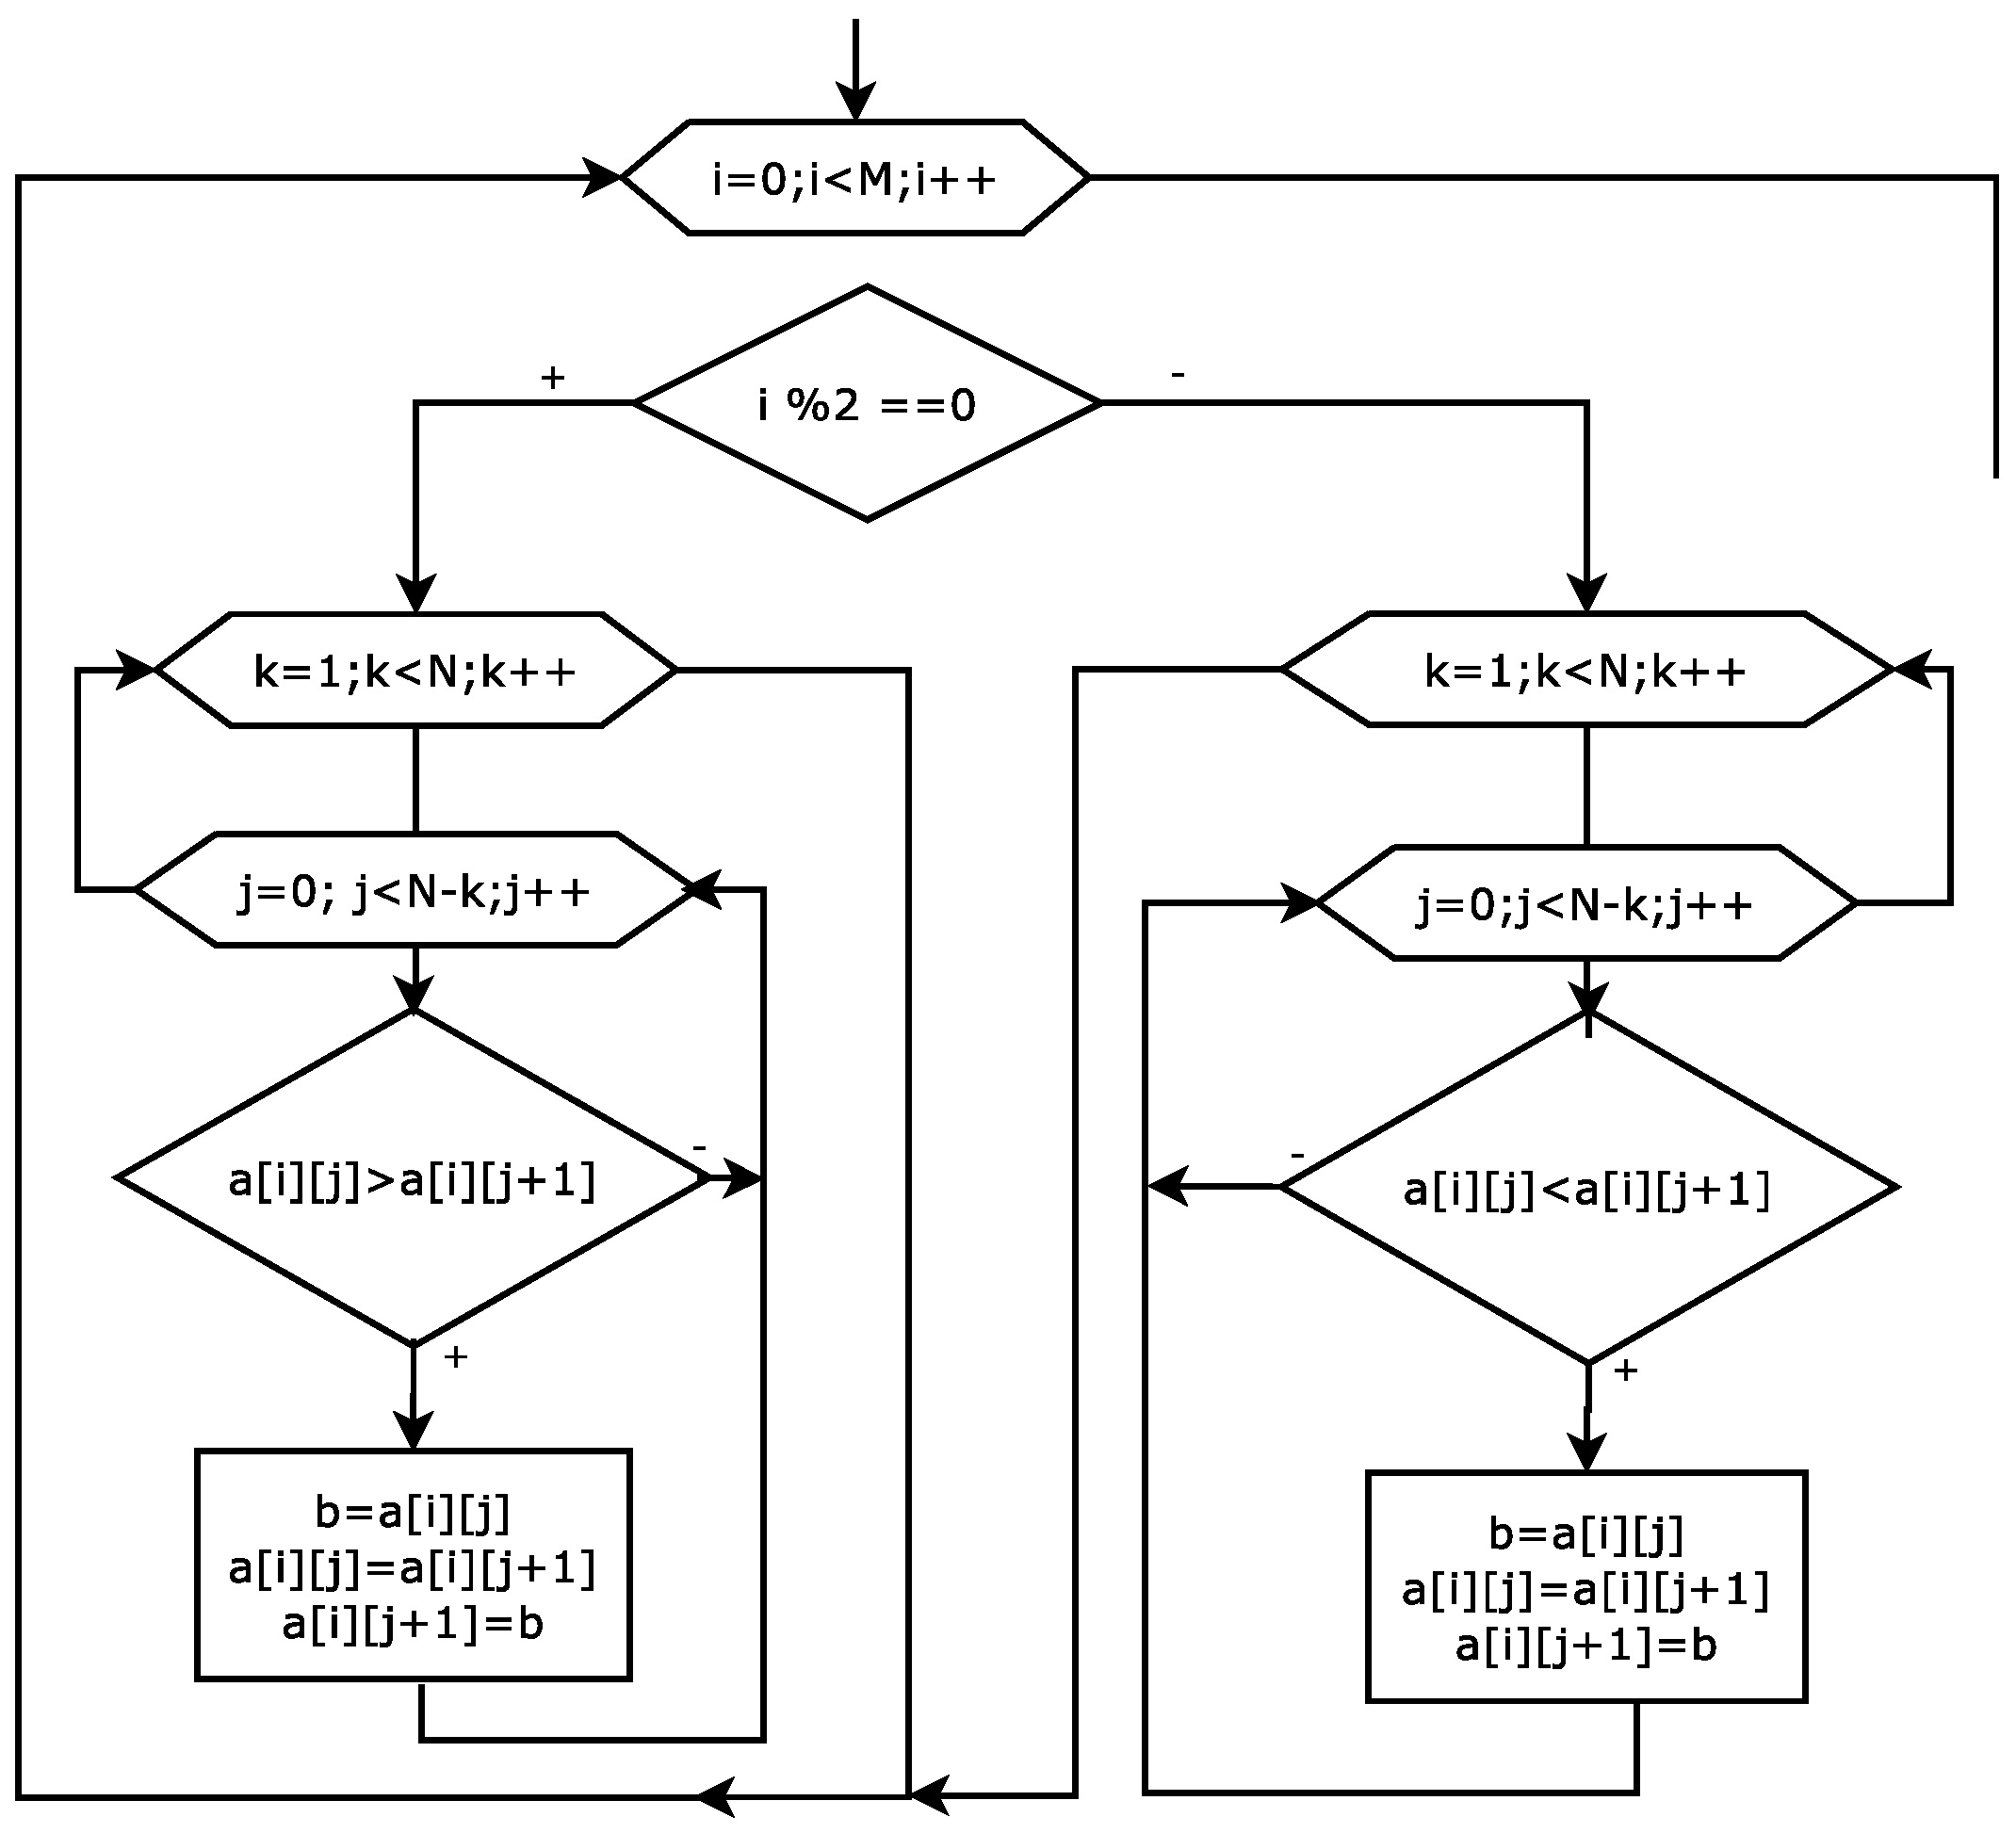
\includegraphics[width=0.7\textwidth]{img/ris_6_10}
\caption{Блок-схема алгоритма задачи~\ref{gl06:prg5}.}
\label{ch06:refDrawing9}
\end{center}
\end{figure}

\begin{lstlisting}
#include <iostream>
using namespace std;
int main()
{
int i,j,k,N,M;
double b, **a; 
//`Ввод размеров матрицы.` 
cout<<"M=";
cin>>M;
cout<<"N=";
cin>>N;
//`Создаём динамическую матрицу`
a=new double *[N];
for(i=0;i<N;i++)
  a[i]=new double [M];
cout<<"`\Sys{Ввод элементов матрицы}` A"<<endl;
for(i=0;i<M;i++)
  for(j=0;j<N;j++)
    cin>>a[i][j];
//`Цикл по `i` --- для перебора строк матрицы.`
for(i=0;i<M;i++)
//`Если строка четна, то`
  if(i%2==0)
  {
//`упорядочиваем элементы строки по возрастанию,`
    for(k=1;k<N;k++)
      for(j=0;j<N-k;j++)
        if(a[i][j]>a[i][j+1])
        {
          b=a[i][j];
          a[i][j]=a[i][j+1];
          a[i][j+1]=b;
        }
  }
  else
//`иначе, нечетные строки, упорядочиваем по убыванию.`
    for(k=1;k<N;k++)
      for(j=0;j<N-k;j++)
        if(a[i][j]<a[i][j+1])
        {
          b=a[i][j];
          a[i][j]=a[i][j+1];
          a[i][j+1]=b;
        }
//`Вывод преобразованной матрицы.`
cout<<"`\Sys{Преобразованная матрица}` A"<<endl;
for(i=0;i<M;cout<<endl,i++)
  for(j=0;j<N;j++)
    cout<<a[i][j]<<"\t";
}
\end{lstlisting}

\prg{Поменять местами элементы главной и побочной диагонали матрицы $A(k,k)$.}{gl06:prg6}

Алгоритм решения задачи следующий: перебираем все строки матрицы (цикл по переменной $i$ от $0$ до
$k-1$ в тексте программы), и в каждой строке меняем местами элементы, расположенные на главной и
побочной диагоналях (в $i$-й строке надо поменять местами элементы \Sys{A[i][i]} и \Sys{А[i][k-i-1]}).
Текст программы с комментариями приведён  далее.
\begin{lstlisting}
#include <iostream>
using namespace std;
int main()
{
  int i,j,k;
  double b,**a; 
//`Ввод размера матрицы.`
  cout<<"k=";
  cin>>k;
//`Создаём динамическую матрицу`
  a=new double *[k];
  for(i=0;i<k;i++)
    a[i]=new double [k];
  cout<<"`\Sys{Ввод элементов матрицы}` A"<<endl;
  for(i=0;i<k;i++)
    for(j=0;j<k;j++)
      cin>>a[i][j];
//`Цикл по строкам.`
  for(i=0;i<k;i++)
  {
//`В каждой строке обмен между элементами, лежащими на`
//`главной и побочной диагоналях.`
    b=a[i][i];
    a[i][i]=a[i][k-1-i];
    a[i][k-1-i]=b;
  }
//`Вывод преобразованной матрицы.` 
  cout<<"`\Sys{Преобразованная матрица}` A"<<endl;
  for(i=0;i<k;cout<<endl,i++)
    for(j=0;j<k;j++)
      cout<<a[i][j]<<"\t";
}
\end{lstlisting}

\prg{Заполнить матрицу $A(6,6)$ числами $1$ до  $36$ следующим образом:}{gl06:prg7}

$\left(\begin{matrix}
1&2&3&4&5&6\\
12&11&10&9&8&7\\
13&14&15&16&17&18\\
24&23&22&21&20&19\\
25&26&27&28&29&30\\
36&35&34&33&32&31
\end{matrix}\right)$%}{gl06:prg7}

Последовательно построчно заполняем матрицу возрастающей арифметической последовательностью  $1,2,3,{\dots},36$. Четные
строки заполняем от нулевого элемента к последнему, а нечётные --- от последнего к нулевому. Текст программы приведён
далее.
\begin{lstlisting}
#include <iostream>
using namespace std;
int main(int argc, char **argv)
{
  int **a,n=6,k=0,i,j;
//`Выделяем память для хранения матрицы`
  a=new int *[n];
  for(i=0;i<n;i++)
    a[i]=new int [n];
//`Перебираем все строки матрицы.`
  for(i=0;i<n;i++)
//`Строки с чётными номерами`
    if (i%2==0)
//`Заполняем возрастающей последовательностью чисел слева направо`
      for(j=0;j<n;j++)
        a[i][j]=++k;
//`Строки с нечётными номерами`
    else
//`Заполняем возрастающей последовательностью чисел справа налево`
      for(j=n-1;j>=0;j--)
        a[i][j]=++k;
    cout<<"`\Sys{Вывод матрицы}` A"<<endl;
    for(i=0;i<n; cout<<endl,i++)
      for(j=0;j<n;j++)
        cout<<a[i][j]<<"\t";
  return 0;
}
\end{lstlisting}

\section[Решение некоторых задач линейной алгебры]{Решение некоторых задач линейной алгебры}
В этом параграфе рассмотрим использование матриц при решении таких задач линейной алгебры, как сложение, вычитание и
умножение матриц, решение систем линейных алгебраических уравнений вычисление определителя и обратной матрицы. В
процессе решения подобных задач будут написаны универсальные функции, которые можно использовать при решении матричной
алгебры.

\prg{Заданы четыре матрицы вещественных чисел
$A(N,M)$, $B(N,M)$, $C(M,N)$, $D(M,N)$. Вычислить матрицу  $C=((A+B)(C-D))^2$.}{gl06:prg8} 

Суммой (разностью) матриц одинаковой размерности $A$ и $B$ называется матрица $C$, элементы которой получаются сложением 
$C_{i,j}=A_{i,j}+B_{i,j}$ (вычитанием  $C_{i,j}=A_{i,j}-B_{i,j}$) соответствующих элементов исходных матриц. 

Напомним алгоритм умножения матриц на примере двух матриц 
$$\left(\begin{matrix}a_{0,0}&a_{0,1}&a_{0,2}\\a_{1,0}&a_{1,1}&a_{1,2}\\a_{2,0}&a_{2,1}&a_{2,2}\end{matrix}\right)\cdot
\left(\begin{matrix}b_{0,0}&b_{0,1}\\b_{1,0}&b_{1,1}\\b_{2,0}&b_{2,1}\end{matrix}\right)$$ 
Воспользовавшись правилом «строка на столбец», получим матрицу: 
{\noindent%\footnotesize 
$\left(\begin{matrix}c_{0,0}&c_{0,1}\\c_{1,0}&c_{1,1}\\c_{2,0}&c_{2,1}\end{matrix}\right)=$\\
$=\left(\begin{matrix}a_{0,0}\cdot
b_{0,0}+a_{0,1}\cdot b_{1,0}+a_{0,2}\cdot b_{2,0}&a_{0,0}\cdot b_{0,1}+a_{0,1}\cdot b_{1,1}+a_{0,2}\cdot
b_{2,1}\\a_{1,0}\cdot b_{0,0}+a_{1,1}\cdot b_{1,2}+a_{1,2}\cdot b_{2,1}&a_{1,0}\cdot b_{0,1}+a_{1,1}\cdot
b_{1,1}+a_{1,2}\cdot b_{2,1}\\a_{2,0}\cdot b_{0,0}+a_{2,1}\cdot b_{1,0}+a_{2,2}\cdot b_{2,0}&a_{2,0}\cdot
b_{0,1}+a_{2,1}\cdot b_{1,1}+a_{2,2}\cdot b_{2,1}\end{matrix}\right)$
}
Произведением матриц $A(N,M)$ и $B(M,L)$ является матрица $C(N,L)$, каждый элемент которой  $C_{i,j}$ вычисляется по формуле:

 $C_{i,j}=\sum\limits_{k=0}^{M-1}A_{i,k}B_{k,j}$, где $i = 0, N-1$ и $j = 0, L-1$. 

Операция умножения имеет смысл только в том случае, если количество строк левой матрицы совпадает с количеством столбцов
правой. Кроме того,  $A\cdot B\neq B\cdot A$. 

При решении задачи будем использовать динамические матрицы и двойные указатели, напишем следующие функции

\begin{itemize}
\item \Sys{float **sum\_m(float **A, float **B, int N, int M)} --- функция формирует матрицу, которая является суммой двух
матриц. Здесь \Sys{A}, \Sys{B} --- указатели на исходные матрицы, \Sys{N}, \Sys{M} --- количество строк и столбцов матриц, функция возвращает
указатель на сформированную матрицу, которая является суммой двух матриц $A$ и $B$.
\item \Sys{float **minus\_m(float **A, float **B, int N, int M})  --- функция формирует матрицу, которая является разностью двух
матриц. Здесь \Sys{A}, \Sys{B} --- указатели на исходные матрицы, \Sys{N}, \Sys{M} --- количество строк и столбцов матриц, функция возвращает
указатель на сформированную матрицу, которая является разностью двух матриц $A$ и $B$.
\item \Sys{float **product\_m(float **A, float **B, int N, int M, int L)} --- функция формирует матрицу, которая является
произведением двух матриц. Здесь \Sys{A}, \Sys{B} --- указатели на исходные матрицы. 
Матрица $A$ имеет $N$ строк и $M$ столбцов, матрица $B$ имеет $M$ строка и $L$ столбцов, функция возвращает указатель 
на сформированную матрицу, которая является произведением
двух матриц $A$ и $B$.
\item \Sys{float **create\_m(int N, int M)} --- функция создаёт матрицу, в которой будет $N$ строк и $M$ столбцов, 
осуществляет ввод элементов матрицы, функция возвращает указатель на сформированную матрицу.
\item \Sys{void output\_m(float **A, int N, int M)} --- функция построчного вывода на экран матрицы $A$, которая 
имеет $N$ строк и $M$ столбцов.
\end{itemize}
Далее приведен текст программы с комментариями.
\begin{lstlisting}
#include <iostream>
using namespace std;
//`функция вычисления суммы двух матриц.`
float **sum_m(float **A, float **B, int N, int M)
{
  int i,j;
//`указатель для хранения результирующей матрицы`
  float **temp;
//`выделение памяти для хранения результирующей матрицы`
  temp=new float *[N];
  for(i=0;i<N;i++)
    temp[i]=new float [M];
//`Вычисляем сумму двух матриц`
  for(i=0;i<N;i++)
    for(j=0;j<M;j++)
      temp[i][j]=A[i][j]+B[i][j];	
//`Возвращаем матрицу как двойной указатель`
  return temp;
}
//`функция вычисления разности двух матриц.`
float **minus_m(float **A, float **B, int N, int M)
{int i,j;
//`указатель для хранения результирующей матрицы`
  float **temp;
//`выделение памяти для хранения результирующей матрицы`
  temp=new float *[N];
  for(i=0;i<N;i++)
  temp[i]=new float [M];
//`Вычисляем разность двух матриц`
  for(i=0;i<N;i++)
    for(j=0;j<M;j++)
      temp[i][j]=A[i][j]-B[i][j];	
//`Возвращаем матрицу как двойной указатель`
  return temp;
}
//`функция вычисления произведения двух матриц.`
float **product_m(float **A, float **B, int N, int M, int L)
{
  int i,j,k;
//`указатель для хранения результирующей матрицы`
  float **temp;
//`выделение памяти для хранения результирующей матрицы`
  temp=new float *[N];
  for(i=0;i<N;i++)
    temp[i]=new float [L];
//`Вычисляем произведение двух матриц`
//`Последовательно формируем все элементы матрицы`
  for(i=0;i<N;i++)
    for(j=0;j<L;j++) 
//`Элемент с индексами `i,j` --- скалярное произведение`
//i`-й строки матрицы `A` и `j`-го  столбца матрицы `B
      for(temp[i][j]=k=0;k<M;k++)
        temp[i][j]+=A[i][k]*B[k][j];
//`Возвращаем матрицу как двойной указатель`
  return temp;
}
//`функция создаёт динамическую матрицу вещественных чисел размерности `N` на `M, 
//`в этой же функции осуществляется и ввод элементов матрицы`
float **create_m(int N, int M)
{
  int i,j;
  float **temp;
  temp=new float *[N];
  for(i=0;i<N;i++)
    temp[i]=new float [M];
  cout<<"`\Sys{Ввод матрицы}`\n";
  for(i=0;i<N;i++)
    for(j=0;j<M;j++)
      cin>>temp[i][j];
  return temp;
} 
//`функция осуществляет построчный вывод матрицы `A(N,M)
void output_m(float **A, int N, int M)
{
  int i,j;
//`Цикл по строкам. По окончанию вывода всех элементов строки --- переход на новую строку.`
  for(i=0;i<N;cout<<endl,i++)
//`Цикл по переменной `j,` в котором перебираем строки матрицы`
    for(j=0;j<M;j++)
//`Вывод очередного элемента матрицы и символа табуляции.`
      cout<<A[i][j]<<"\t";
}
int main(int argc, char **argv)
{
//`указатели для хранения исходных и результирующие матрицы`
  float **A, **B, **C, **D,**result;
  int N,M; 
//`Ввод размерностей матрицы`
  cout<<"N=";cin>>N;
  cout<<"M=";cin>>M;
//`Выделение памяти и ввод матриц `A, B, C, D,` обращаясь к функции `create_m.
  A=create_m(N,M);
  B=create_m(N,M);
  C=create_m(M,N);
  D=create_m(M,N);
//`Вычисление результирующей матрицы.`
  result=product_m(product_m(sum_m(A,B,N,M), minus_m(C,D,M,N),N,M,N), product_m(sum_m(A,B,N,M), minus_m(C,D,M,N),N,M,N),N,N,N);
//`Вывод результирующей матрицы.`
  output_m(result,N,N);
  return 0;
}
\end{lstlisting}

Далее без комментариев приведена программа решения задачи~\ref{gl06:prg8} с помощью динамических матриц и обычных
указателей\footnote{Обращаем внимание читателя, что при использовании одинарных указателей обращение к элементам
матрицы происходит быстрее. При обработке матриц большой размерности (более 1000000 элементов) имеет смысл использовать
именно одинарные указатели для хранения и обработки матриц. Это позволит ускорить работу программ на 10-15\%.}.
Рекомендуем читателям самостоятельно разобраться с этой версией программы.
\begin{lstlisting}
#include <iostream>
using namespace std;
float *sum_m(float *A, float *B, int N, int M)
{
  int i,j;
  float *temp;
  temp=new float [N*M];
  for(i=0;i<N;i++)
    for(j=0;j<M;j++)
      temp[i*M+j]=A[i*M+j]+B[i*M+j];	
  return temp;
}
float *minus_m(float *A, float *B, int N, int M)
{int i,j;
  float *temp;
  temp=new float [N*M];
  for(i=0;i<N;i++)
    for(j=0;j<M;j++)
      temp[i*M+j]=A[i*M+j]-B[i*M+j];	
  return temp;
}
float *product_m(float *A, float *B, int N, int M, int L)
{
  int i,j,k;
  float *temp;
  temp=new float [N*L];
  for(i=0;i<N;i++)
    for(j=0;j<L;j++)
      for(temp[i*L+j]=k=0;k<M;k++)
        temp[i*L+j]+=A[i*M+k]*B[k*L+j];	
  return temp;
}
float *create_m(int N, int M)
{
  int i,j;
  float *temp;
  temp=new float [N*M];
  cout<<"`\Sys{Ввод матрицы}`\n";
  for(i=0;i<N;i++)
    for(j=0;j<M;j++)
      cin>>temp[i*M+j];
  return temp;
} 
void output_m(float *A, int N, int M)
{
  int i,j;
  for(i=0;i<N;cout<<endl,i++)
    for(j=0;j<M;j++)
      cout<<A[i*M+j]<<"\t";
}
int main(int argc, char **argv)
{
  float *A, *B, *C, *D,*result;
  int N,M;
  cout<<"N=";cin>>N;
  cout<<"M=";cin>>M;
  A=create_m(N,M);
  B=create_m(N,M);
  C=create_m(M,N);
  D=create_m(M,N);
  result=product_m(product_m(sum_m(A,B,N,M), minus_m(C,D,M,N),N,M,N), product_m(sum_m(A,B,N,M), minus_m(C,D,M,N),N,M,N),N,N,N);
  output_m(result,N,N);
  return 0;
}
\end{lstlisting}

\prg{Решить систему линейных алгебраических уравнений.}{gl06:prg9}

При решении этой задачи напишем универсальную функцию решения системы 
линейных алгебраических уравнений методом Гаусса, а
в функции \Sys{main()} просто вызовем эту функцию. Вспомним метод Гаусса.

Пусть дана система линейных алгебраических уравнений (СЛАУ) с $n$ неизвестными 

\begin{equation}\label{gl06:prg0a}
\left\{\begin{array}{ll}
a_{00}x_0+a_{01}x_1+...+a_{0n-1}x_{n-1}&=b_0,\\
a_{10}x_0+a_{11}x_1+...+a_{1n-1}x_{n-1}&=b_1,\\
\hdotsfor{2}\\
a_{n-10}x_0+a_{n-11}x_1+...+a_{n-1n-1}x_{n-1}&=b_{n-1}
\end{array}\right.
\end{equation}
Обозначим через 
$A=\left(\begin{matrix}
a_{00}&a_{01}&...&a_{0n-1}\\
a_{10}&a_{11}&...&a_{1n-1}\\
...&...&...&...\\
a_{n-10}&a_{n-11}&...&a_{n-1n-1}
\end{matrix}\right)$
матрицу коэффициентов системы (\ref{gl06:prg0a}), через 
$b=\left(\begin{matrix}b_0\\b_1\\...\\b_{n-1}\end{matrix}\right)$ --- столбец ее свободных членов, и через
$x=\left(\begin{matrix}x_0\\x_1\\...\\x_{n-1}\end{matrix}\right)$ --- столбец из неизвестных (искомый вектор). Тогда
система (\ref{gl06:prg0a})  может быть записана в виде матричного уравнения  $Ax=b$.

Наиболее распространенным приёмом решения систем линейных уравнений\index{Метод Гаусса!решение систем линейных
уравнений} является алгоритм последовательного исключения неизвестных --- \emph{метод Гаусса}.

При решении систем линейных алгебраических уравнений этим методом всевозможные преобразования производят не над
уравнениями системы (\ref{gl06:prg0a}), а над так называемой \emph{расширенной матрицей} системы, которая получается
путём добавления к основной матрице $A$ столбца свободных членов $b$.

Первый этап решения системы уравнений, называемый \emph{прямым ходом метода Гаусса}, заключается в приведении
расширенной матрицы (\ref{gl06:prg1a}) к \emph{треугольному виду}. Это означает, что все элементы матрицы
(\ref{gl06:prg1a}) ниже главной диагонали должны быть равны нулю.

\begin{equation}\label{gl06:prg1a}
A'=\left(\begin{matrix}
a_{00}&a_{01}&...&a_{0n-1}&b_0\\
a_{10}&a_{11}&...&a_{1n-1}&b_1\\
...&...&...&...&...\\
a_{n-10}&a_{n-11}&...&a_{n-1n-1}&b_{n-1}
\end{matrix}\right)
\end{equation}

На первом этапе необходимо обнулить элементы 0-го столбца расширенной матрицы 

\begin{equation}\label{gl06:prg2a}
A^{'}=\left(\begin{matrix}
a_{00}&a_{01}&a_{02}&...&a_{0n-1}&b_0\\
0&a_{11}&a_{12}&...&a_{1n-1}&b_1\\
0&0&a_{22}&...&a_{2n-1}&b_2\\
0&0&0&...&a_{3n-1}&b_3\\
...&...&...&...&...&...\\
0&0&0&...&a_{n-1n-1}&b_{n-1}
\end{matrix}\right)
\end{equation}

Для этого необходимо из каждой строки (начиная со первой) вычесть нулевую, умноженную на некоторое число $M$. В
общем виде этот процесс можно записать так:

1-я строка = 1-я строка -- $M\times$ 0-я строка

2-я строка = 2-я строка -- $M\times$ 0-я строка

…

$i$-я строка = $i$-я строка -- $M\times$ 0-я строка

…

$n-1$-я строка = $n-1$-я строка -- $M\times$ 0-я строка

Понятно, что преобразование элементов первой строки будет происходить по формулам:\\
$a_{10}=a_{10}-Ma_{00}$ \\
$a_{11}=a_{11}-Ma_{01}$\\
 …  \\
$a_{1i}=a_{1i}-Ma_{0i}$\\
 … \\
$a_{1n-1}=a_{1n-1}-Ma_{0n-1}$\\
$b_1=b_1-Mb_0$ 

Так как целью данных преобразований является обнуление первого элемента строки, то $M$ выбираем из условия: 
$a_{10}=a_{10}-Ma_{00}=0$. Следовательно,  $M=\frac{a_{10}}{a_{00}}$.

Элементы второй строки и коэффициент $M$ можно рассчитать аналогично:\\
$a_{20}=a_{20}-Ma_{00}$\\
$a_{21}=a_{21}-Ma_{01}$\\
…\\
$a_{1i}=a_{1i}-Ma_{0i}$\\
… \\
$a_{2n-1}=a_{2n-1}-Ma_{0n-1}$\\  
$b_2=b_2-Mb_0$\\
$a_{20}=a_{20}-Ma_{00}=0 \Rightarrow M=\frac{a_{20}}{a_{00}}$.

Таким образом, преобразование элементов $i$–й строки будет происходить следующим образом:\\
$a_{i0}=a_{i0}-Ma_{00}$\\  
$a_{i1}=a_{i1}-Ma_{01}$\\ 
…\\ 
$a_{ii}=a_{ii}-Ma_{0i}$\\
 …\\  
$a_{in-1}=a_{in-1}-Ma_{0n-1}$\\
$b_i=b_i-Mb_0$.

Коэффициент $M$ для $i$–й строки выбирается из условия
$a_{i0}=a_{i0}-Ma_{00}=0$
и равен 
 $M=\frac{a_{i0}}{a_{00}}$.

После проведения подобных преобразований для всех строк матрица (\ref{gl06:prg1a}) примет вид

$A'=\left(\begin{matrix}a_{00}&a_{01}&...&a_{0n-1}&b_0\\0&a_{11}&...&a_{1n-1}&b_1\\0&a_{21}&...&a_{2n-1}&b_2\\...&...&...&...&...\\0&a_{n-11}&...&a_{n-1n-1}&b_{n-1}\end{matrix}\right)$.

Блок-схема обнуления первого столбца матрицы приведена на рис.~\ref{ch06:refDrawing10}.

Очевидно, что если повторить описанный выше алгоритм для следующих столбцов матрицы (\ref{gl06:prg1a}), причём начинать
преобразовывать первый столбец со второго элемента, второй столбец --- с третьего и т.д., то в результате будет получена
матрица (\ref{gl06:prg2}). Алгоритм этого процесса изображён на рис.~\ref{ch06:refDrawing11}.
%%%%%%%%%%%%%%%%%%%%%%
%%%% рис 6.11 и 6.12 бок о бок
{\small
\begin{figure}[H]
\begin{floatrow}
\floatbox{figure}[.45\textwidth][\FBheight][t]
{\caption{Блок-схема обнуления первого столбца матрицы}
\label{ch06:refDrawing10}}
{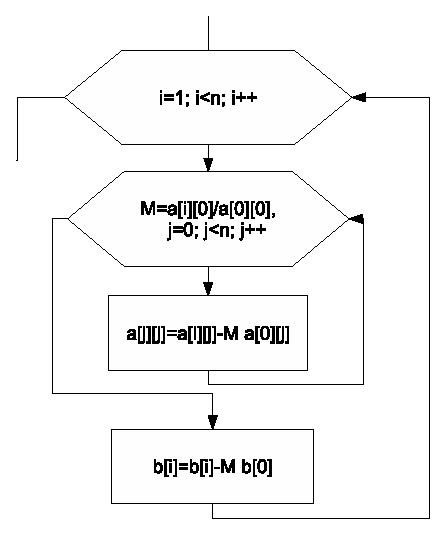
\includegraphics[width=0.45\textwidth,keepaspectratio]{img/ris_6_11}}\hspace*{0.05\textwidth}
%
\floatbox{figure}[.45\textwidth][\FBheight][b]
{\caption{Блок-схема алгоритма преобразования расширенной матрицы к треугольному виду}
\label{ch06:refDrawing11}}
{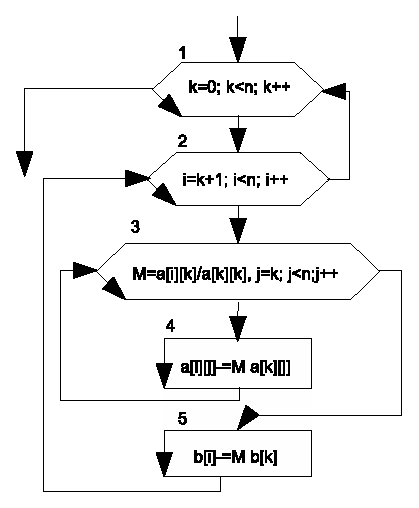
\includegraphics[width=0.45\textwidth,keepaspectratio]{img/ris_6_12}}
\end{floatrow}
\end{figure}
}
%%%%%%%%%%%%%%%%%%%%%%%%

Заметим, что если в матрице (\ref{gl06:prg1a}) на главной диагонали встретится элемент  $a_{k,k}$, равный нулю, то
расчёт коэффициента $M=\frac{a_{ik}}{a_{kk}}$  для $k$-й строки будет невозможен. Избежать деления на
ноль можно, избавившись от нулевых элементов на главной диагонали. Для этого перед обнулением элементов в $k$–м столбце
необходимо найти в нем максимальный по модулю элемент (среди расположенных ниже  $a_{k,k}$, запомнить номер строки, в
которой он находится, и поменять ее местами с $k$-й. Алгоритм, отображающий эти преобразования, приведён 
на рис.~\ref{ch06:refDrawing12}.

В результате выполнения прямого хода метода Гаусса матрица (\ref{gl06:prg1a}) преобразуется в матрицу (\ref{gl06:prg2a}), а
система уравнений (\ref{gl06:prg0a}) будет иметь следующий вид:

\begin{equation}\label{gl06:prg3a}
\left\{\begin{matrix}
a_{00}x_0+a_{01}x_1+a_{20}x_2+...+a_{0n-1}x_{n-1}&=b_0,\\
a_{11}x_1+a_{21}x_2+...+a_{1n-1}x_{n-1}&=b_1,\\
a_{22}x_2+...+a_{2n-1}x_{n-1}&=b_2,\\
...\\
a_{n-1n-1}x_{n-1}&=b_{n-1}
\end{matrix}\right.
\end{equation}



%\begin{figure}[htb]
%\begin{center}
%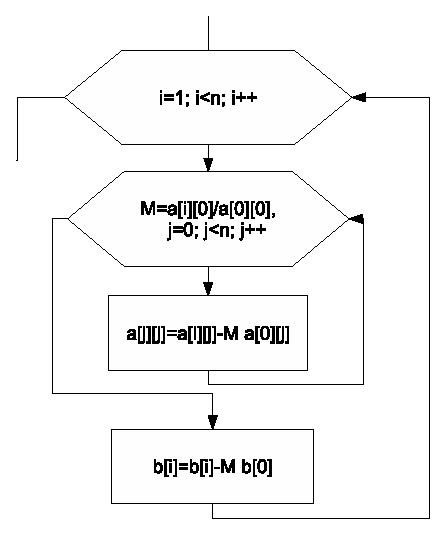
\includegraphics[width=0.5\textwidth]{img/ris_6_11}
%\caption{Блок-схема обнуления первого столбца матрицы}
%\label{ch06:refDrawing10}
%\end{center}
%\end{figure}

Решение системы (\ref{gl06:prg3}) называют \emph{обратным ходом метода Гаусса}.

Последнее $(n-1)$-е уравнение системы (\ref{gl06:prg3}) имеет вид:
 $a_{n-1n-1}x_{n-1}=b_{n-1}$.
Тогда, если  $a_{n-1n-1}\neq 0$, то  $x_{n-1}=\frac{b_{n-1}}{a_{n-1n-1}}$. 
В случае, если  $a_{n-1n-1}=0,$ и $b_{n-1}=0$, то система (\ref{gl06:prg3a}), 
а следовательно, и система (\ref{gl06:prg0a}) имеют бесконечное множество
решений. 

При  $a_{n-1n-1}=0,$ и  $b_{n-1}\neq 0$  система (\ref{gl06:prg3}), а значит, и система (\ref{gl06:prg0a}) решения не
имеет.
Предпоследнее $(n-2)$-е уравнение системы (\ref{gl06:prg3a}) имеет вид
$a_{n-2n-2}x_{n-2}+a_{n-2n-1}x_{n-1}=b_{n-2}$.

%\begin{figure}[htb]
%\begin{center}
%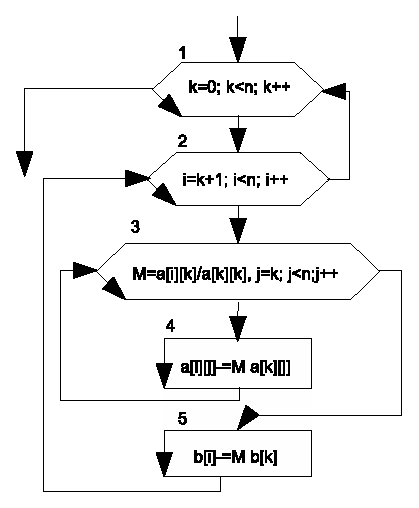
\includegraphics[width=0.5\textwidth]{img/ris_6_12}
%\caption{Блок-схема алгоритма преобразования расширенной матрицы к треугольному виду}
%\label{ch06:refDrawing11}
%\end{center}
%\end{figure}


%\begin{figure}[htb]
%\begin{center}
%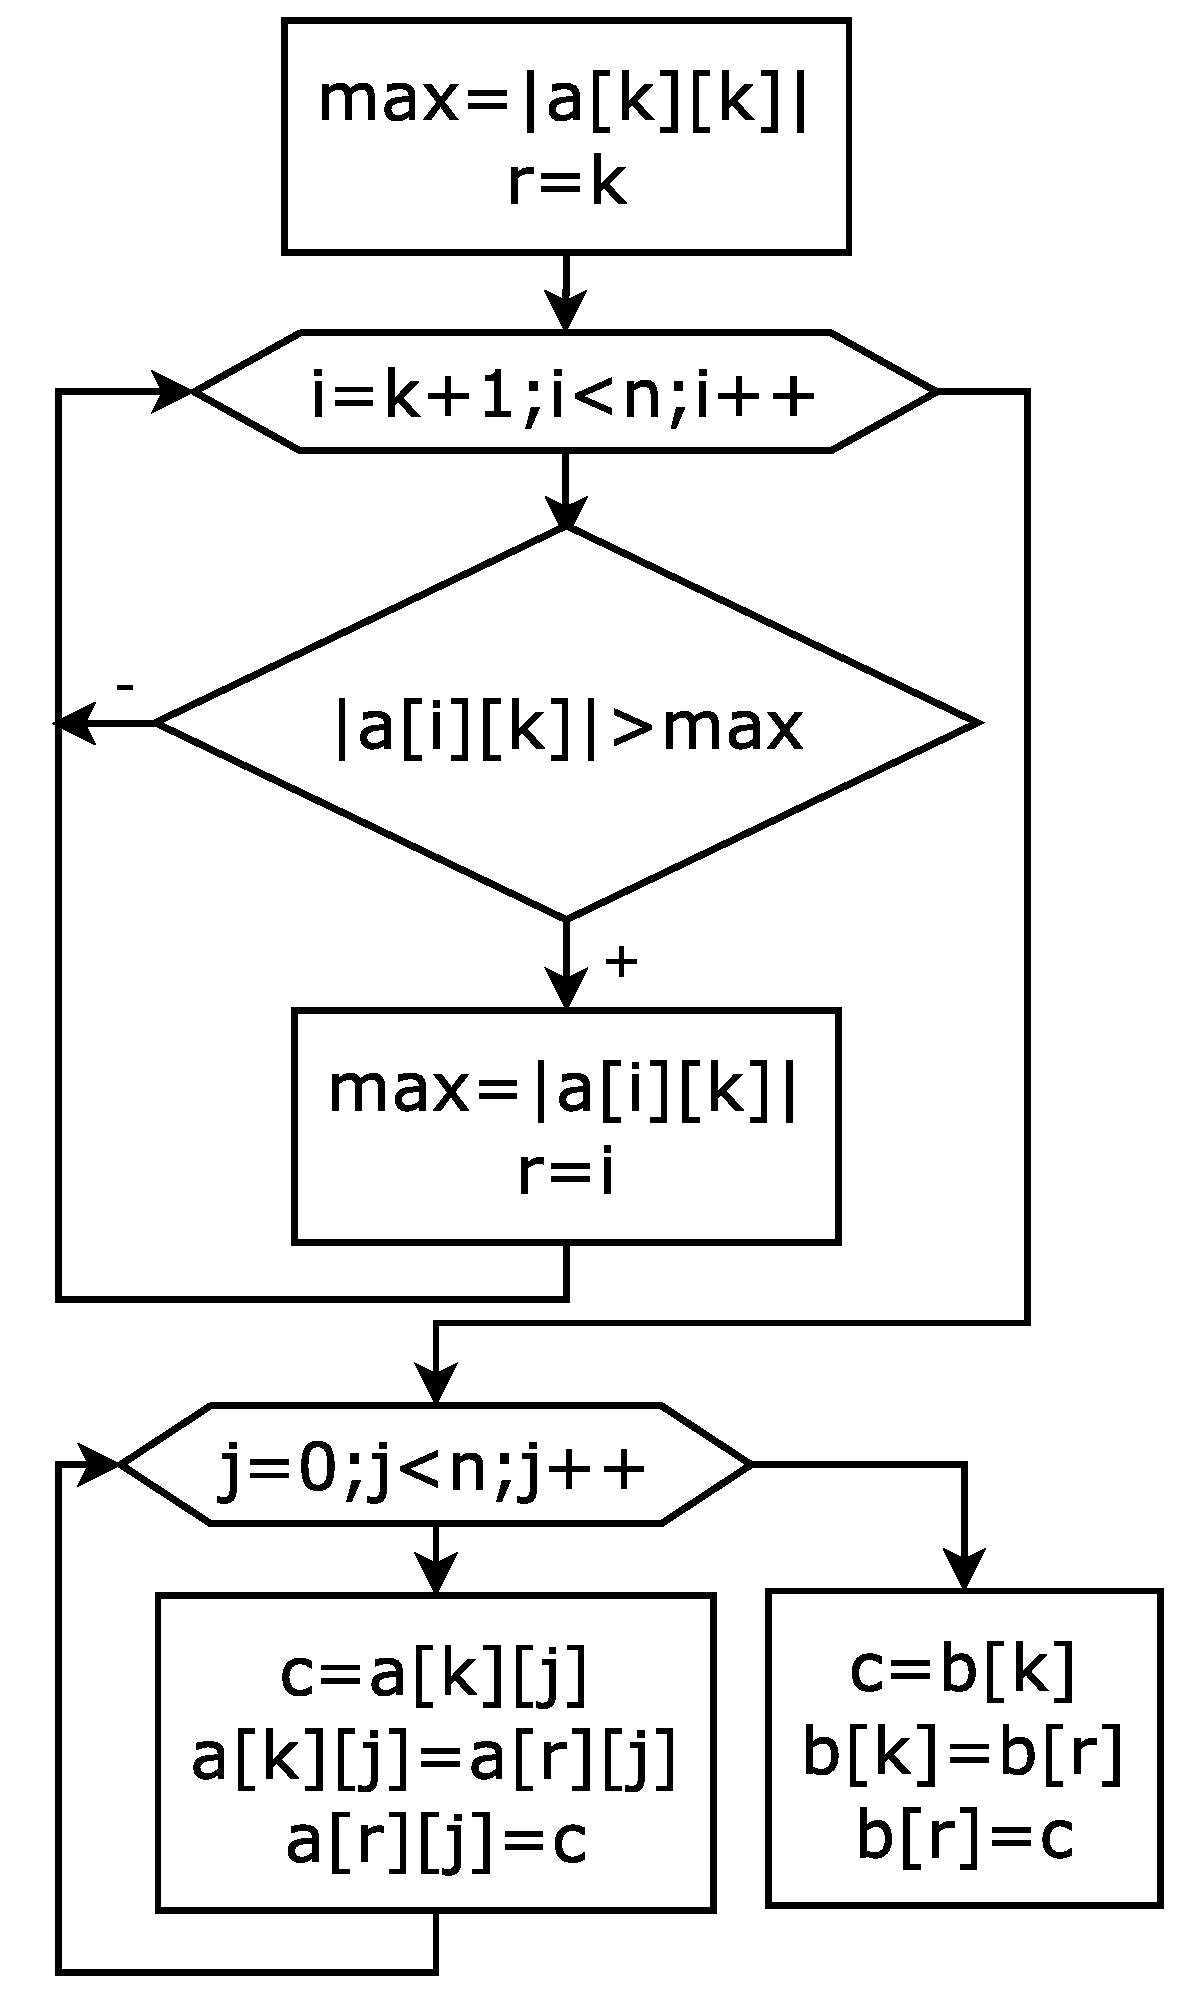
\includegraphics[width=0.5\textwidth]{img/ris_6_13}
%\caption{Блок-схема алгоритма перестановки строк расширенной матрицы}
%\label{ch06:refDrawing12}
%\end{center}
%\end{figure}
%%%%%%%%%%%%%%%%%%%%%%
%%%% рис 6.13 и 6.14 бок о бок
\begin{figure}[H]
\begin{floatrow}
\floatbox{figure}[.45\textwidth][\FBheight][t]
{\caption{Блок-схема алгоритма перестановки строк расширенной матрицы}
\label{ch06:refDrawing12}}
{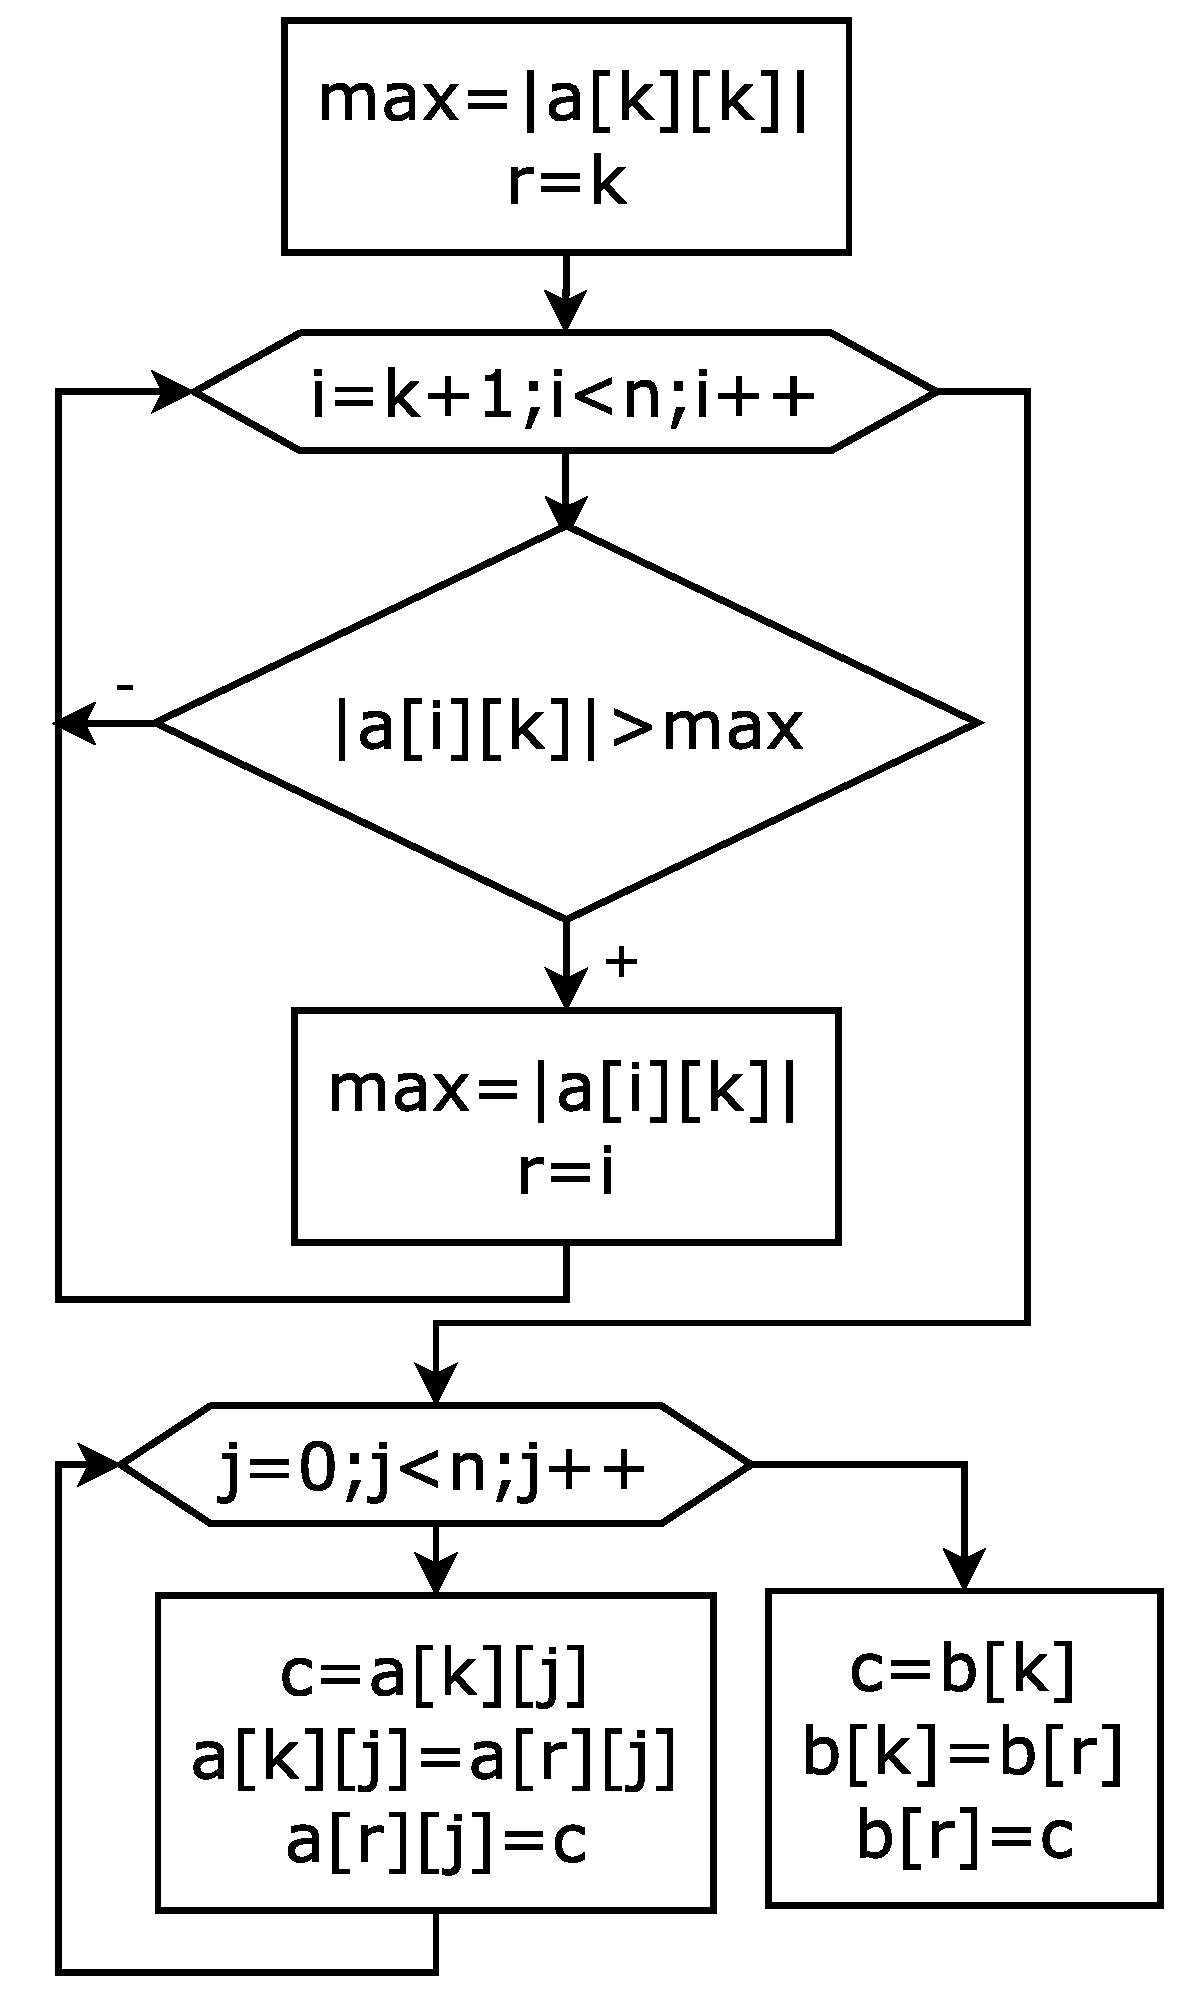
\includegraphics[width=0.45\textwidth,keepaspectratio]{img/ris_6_13}}\hspace*{0.05\textwidth}
%
\floatbox{figure}[.45\textwidth][\FBheight][b]
{\caption{Блок-схема алгоритма обратного хода метода Гаусса}
\label{ch06:refDrawing13}}
{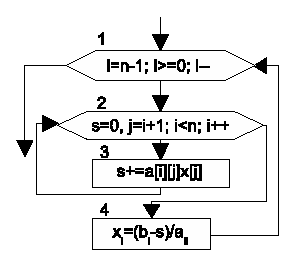
\includegraphics[width=0.45\textwidth,keepaspectratio]{img/ris_6_14}}
\end{floatrow}
\end{figure}
%%%%%%%%%%%%%%%%%%%%%%%%



Значит, $x_{n-2}=\frac{b_{n-2}-a_{n-2n-1}x_{n-1}}{a_{n-2n-2}}$.

Следующее $(n-3)$-е уравнение системы (\ref{gl06:prg3}) будет выглядеть так:

 $a_{n-3n-3}x_{n-3}+a_{n-3n-2}x_{n-2}+a_{n-3n-1}x_{n-1}=b_{n-3}$.

Отсюда имеем

 $x_{n-3}=\frac{b_{n-3}-a_{n-3n-2}x_{n-2}-a_{n-3n-1}x_{n-1}}{a_{n-3n-3}},x_{n-3}=
\frac{b_{n-3}-\sum\limits_{j=n-2}^{n-1}{a_{n-3j}x_j}}{a_{n-3n-3}}$.

Таким образом, формула для вычисления $i$-го значения $x$ будет иметь вид:
$x_i=\frac{b_i-\sum\limits_{j=i+1}^{n-1}{a_{ij}x_j}}{a_{ii}}$.

Алгоритм, реализующий обратный ход метода Гаусса, представлен в виде блок-схемы на рис.~\ref{ch06:refDrawing13}.

% [Warning: Image ignored] % Unhandled or unsupported graphics:
%\captionof{figure}[Блок{}-схема алгоритма обратного хода метода Гаусса ]{Блок-схема алгоритма обратного хода метода
%Гаусса }
%\label{ch06:refDrawing13}


Объединив блок-схемы, изображенные на рис.~\ref{ch06:refDrawing11}, \ref{ch06:refDrawing12} и \ref{ch06:refDrawing13},
получим общую блок-схему метода Гаусса (рис.~\ref{ch06:refDrawing14}). Блоки 2-6 содержат последовательный ввод данных,
где $n$ --- это размерность системы линейных алгебраических уравнений, а сама система задаётся в виде матрицы коэффициентов
при неизвестных $A$ и вектора свободных коэффициентов $b$. Блоки 7-18 предусматривают прямой ход метода Гаусса, а блоки
23-27 --- обратный. Для вывода результатов предусмотрено несколько блоков вывода. Если результат проверки условий 19 и 20
положительный, то выдается сообщение о том, что система имеет бесконечное множество решений (блок 21). Если условие 19
выполняется, а 20 --- нет, то появляется сообщение о том, что система не имеет решений (блок 22). Сами же решения системы
уравнений, представленные вектором $x$, вычисляются (блоки 23–26) и выводятся экран печать (блок 27) только в случае
невыполнения условия.

Теперь алгоритм решения СЛАУ, представленный на рис.~\ref{ch06:refDrawing14} разобьём на главную функцию \Sys{main()}
и функцию решения СЛАУ методом Гаусса. В функции \Sys{main()} будет находиться ввод исходных данных, обращение к
функции SLAU решения системы линейных алгебраических уравнений и вывод вектора решения. Функция SLAU предназначена для
решения системы линейных алгебраических уравнений методом Гаусса.

\begin{figure}[htb]
\begin{center}
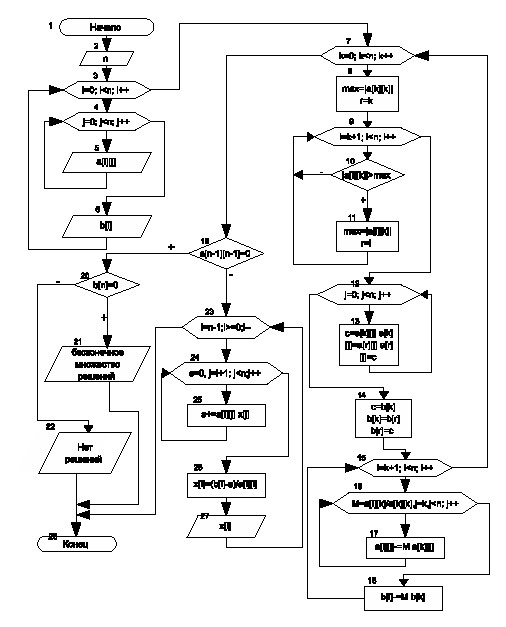
\includegraphics[width=0.8\textwidth]{img/ris_6_15}
\caption{Блок-схема алгоритма решения СЛАУ методом Гаусса}
\label{ch06:refDrawing14}
\end{center}
\end{figure}

При написании функции следует учитывать следующее: в методе Гаусса изменяются матрица коэффициентов и вектор правых
частей. Поэтому, для того чтобы их не испортить, в функции SLAU матрицу коэффициентов и вектор правых частей необходимо
скопировать во внутренние переменные, и в функции обрабатывать внутренние переменные-копии.

Функция \Sys{SLAU} возвращает значение 0, если решение найдено, $-1$ --- если система имеет 
бесконечное множество решений, $-2$ --- если система не имеет решений.

Ниже приведено решение задачи~\ref{gl06:prg9} с подробными комментариями.
\begin{lstlisting}
#include <iostream>
#include <math.h>
using namespace std;
int SLAU(double **matrica_a,  int n, double *massiv_b, double *x)
//`Функция SLAU возвращает значение типа int:`
//`0, если решение найдено, -1 --- если система имеет бесконечное множество` 
//`решений, -2 --- если система не имеет решений.`
//`Формальные параметры функции: `n` --- размерность системы, `matrica_a 
//`---  матрица коэффициентов СЛАУ,` massiv_b `--- вектор правых частей, `
//x` --- решение СЛАУ,` a, b, x` передаются как указатели.`
{
  int i,j,k,r;
  double c,M,max,s;
//`Матрица a --- копия матрицы коэффициентов,` 
//`массив b --- копия вектора правых частей.`
  double **a, *b; 
//`Выделение памяти для a и b.`
  a=new double *[n];
  for(i=0;i<n;i++)
    a[i]=new double[n];
  b=new double [n];
//`В a записываем копию матрицы коэффициентов,`
//b `копию вектора правых частей.`
  for(i=0;i<n;i++)
    for(j=0;j<n;j++)
      a[i][j]=matrica_a[i][j];
      for(i=0;i<n;i++)
        b[i]=massiv_b[i];
//`Прямой ход метода Гаусса: приводим матрицу a` 
//`(копию матрицы коэффициентов СЛАУ) к диагональному виду.`
  for(k=0;k<n;k++)
  {
//`Поиск максимального по модулю элемента в k-м столбце.`
    max=fabs(a[k][k]);
    r=k;
    for(i=k+1;i<n;i++)
      if (fabs(a[i][k])>max)
      {
        max=fabs(a[i][k]);
        r=i;
      }
//`Меняем местами k-ю и r-ю (строку, где находится` 
//`максимальный по модулю элемент) строки.`
    for(j=0;j<n;j++)
    {
      c=a[k][j];
      a[k][j]=a[r][j];
      a[r][j]=c;
    }
    c=b[k];
    b[k]=b[r];
    b[r]=c;
//`Приведение матрицы к диагональному виду.`
    for(i=k+1;i<n;i++)
    {
      for(M=a[i][k]/a[k][k],j=k;j<n;j++)
        a[i][j]-=M*a[k][j];
        b[i]-=M*b[k];
    }
  }
//`Обратный ход метода Гаусса.`
//`Если последний диагональный элемент равен 0 и` 
  if (a[n-1][n-1]==0)
//`если последний коэффициент вектора свободных членов равен 0,`
    if(b[n-1]==0)
//`то система имеет бесконечное множество решений`
      return -1;
//`если последний коэффициент вектора свободных членов не`
//`равен 0, то система решений не имеет.`
    else return -2;
  else
//`Если последний диагональный элемент не равен 0, то` 
//`начинается обратный ход метода Гаусса.`
  {
    for(i=n-1;i>=0;i--)
    {
      for(s=0,j=i+1;j<n;j++)
        s+=a[i][j]*x[j];
      x[i]=(b[i]-s)/a[i][i];
    }
    return 0;
  }	
}
int main()
{
  int result,i,j,N;
  double **a, *b, *x; 
//`Ввод размерности системы.`
  cout<<"N=";
  cin>>N;
//`Выделение памяти для матрицы правых частей и вектора свободных членов.`
  a=new double *[N];
  for(i=0;i<N;i++)
    a[i]=new double[N];
  b=new double [N];
  x=new double [N];
//`Ввод матрицы правых частей и вектора свободных членов.`
  cout<<"`\Sys{Ввод матрицы}` A"<<endl;
  for(i=0;i<N;i++)
    for(j=0;j<N;j++)
      cin>>a[i][j];
  cout<<"`\Sys{Ввод вектора}` B"<<endl;
  for(i=0;i<N;i++)
    cin>>b[i];
//`Вызов функции решения СЛАУ методом Гаусса. По значению`
//`переменной result можно судить, сколько корней имеет`
//`система. Если result=0, то  система имеет единственное`
//`решение, result= -1, то система имеет бесконечное`
//`множество решений, result=-2, система не имеет решений.`
  result=SLAU(a,N,b,x);
  if (result==0)
  {
//`Вывод массива решения.`
    cout<<"Massiv X"<<endl;
    for(i=0;i<N;i++)
      cout<<x[i]<<"\t";
    cout<<endl;
  }
  else if (result==-1)
    cout<<"`\Sys{Бесконечное множество решений}`\n";
       else if (result==-2)
         cout<<"`\Sys{Нет решений}`\n";
}
\end{lstlisting}

\prg{Найти обратную матрицу к квадратной матрицы $A(N,N)$.}{gl06:prg10}

Один из методов вычисления \emph{обратной матрицы}\index{Метод Гаусса!вычисление обратной матрицы} основан на решении
систем линейных алгебраических уравнений. Пусть задана некоторая матрица A:

\begin{equation}\label{gl06:prg4a}
A=\left(\begin{matrix}a_{00}&a_{01}&a_{02}&...&a_{0n-1}\\a_{10}&a_{11}&a_{12}&...&a_{1n-1}\\...&...&...&...&...\\a_{n-10}&a_{n-11}&a_{n-12}&...&a_{n-1n-1}\end{matrix}\right)
\end{equation}
Необходимо найти матрицу $A^{-1}$, которая является обратной к матрице $A$:

\begin{equation}\label{gl06:prg5a}
Y=A^{-1}=\left(\begin{matrix}y_{00}&y_{01}&y_{02}&...&y_{0n-1}\\y_{10}&y_{11}&y_{12}&...&y_{1n-1}\\...&...&...&...&...\\y_{n-10}&y_{n-11}&y_{n-12}&...&y_{n-1n-1}\end{matrix}\right)
\end{equation}
Матрица (\ref{gl06:prg5a}) будет обратной к матрице (\ref{gl06:prg4a}), если выполняется соотношение $A\cdot A^{-1}=E$,
где Е --- это единичная матрица, или более подробно:

\noindent\begin{equation}\label{gl06:prg6a}
\left(\begin{matrix}a_{00}&a_{01}&...&a_{0n-1}\\a_{10}&a_{11}&...&a_{1n-1}\\...&...&...&...\\a_{n-10}&a_{n-11}&...&a_{n-1n-1}\end{matrix}\right)\left(\begin{matrix}y_{00}&y_{01}&...&y_{0n-1}\\y_{10}&y_{11}&...&y_{1n-1}\\...&...&...&...\\y_{n-10}&y_{n-11}&...&y_{n-1n-1}\end{matrix}\right)=E
\end{equation}
Результат перемножения матриц из соотношения (\ref{gl06:prg6a}) можно представить поэлементно в виде n систем линейных
уравнений. Умножение матрицы (\ref{gl06:prg4a}) на нулевой столбец матрицы (\ref{gl06:prg5a}) даст нулевой столбец
единичной матрицы:

$\left\{\begin{matrix}
a_{00}y_{00}+a_{01}y_{10}+...+a_{0n-1}y_{n-10}&=1,\\
a_{10}y_{00}+a_{11}y_{10}+...+a_{1n-1}y_{n-10}&=0,\\
\hdotsfor{2}\\
a_{i0}y_{00}+a_{i1}y_{10}+...+a_{in-1}y_{n-10}&=0,\\
\hdotsfor{2}\\
a_{n-10}y_{00}+a_{n-11}y_{10}+...+a_{n-1n-1}y_{n-10}&=0
\end{matrix}\right.$.

При умножении матрицы $A$ на второй столбец обратной матрицы получается следующая система линейных алгебраический
уравнений.

\begin{equation*}
\left\{\begin{matrix}
a_{00}y_{01}+a_{01}y_{11}+...+a_{0n-1}y_{n-11}&=0,\\
a_{10}y_{01}+a_{11}y_{11}+...+a_{1n-1}y_{n-11}&=1,\\
\hdotsfor{2}\\
a_{i0}y_{01}+a_{i1}y_{11}+...+a_{in-1}y_{n-11}&=0,\\
\hdotsfor{2}\\
a_{n-10}y_{01}+a_{n-11}y_{11}+...+a_{n-1n-1}y_{n-11}&=0
\end{matrix}\right.
\end{equation*}
Система, полученная в результате умножения матрицы (\ref{gl06:prg4a}) на $i$-й столбец матрицы
(\ref{gl06:prg5a}), будет выглядеть следующим образом:

\begin{equation*}
\left\{\begin{matrix}
a_{00}y_{0i}+a_{01}y_{1i}+...+a_{0n-1}y_{n-1i}&=0,\\
a_{10}y_{0i}+a_{11}y_{1i}+...+a_{1n-1}y_{n-1i}&=0,\\
\hdotsfor{2}\\
a_{i0}y_{0i}+a_{i1}y_{1i}+...+a_{in-1}y_{n-1i}&=1,\\
\hdotsfor{2}\\
a_{n-10}y_{0i}+a_{n-11}y_{1i}+...+a_{n-1n-1}y_{n-1i}&=0
\end{matrix}\right.
\end{equation*}
Понятно, что $n$-я система будет иметь вид:

$\left\{\begin{matrix}
a_{00}y_{0n-1}+a_{01}y_{1n-1}+...+a_{0n-1}y_{n-1n-1}&=0,\\
a_{10}y_{0n-1}+a_{11}y_{1n-1}+...+a_{1n-1}y_{n-1n-1}&=0,\\
\hdotsfor{2}\\
a_{i0}y_{0n-1}+a_{i1}y_{1n-1}+...+a_{in-1}y_{n-1n-1}&=0,\\
\hdotsfor{2}\\
a_{n-10}y_{0n-1}+a_{n-11}y_{1n-1}+...+a_{n-1n-1}y_{n-1n-1}&=1
\end{matrix}\right.$.

Решением каждой из приведенных выше систем будет $i$-й столбец обратной матрицы. Количество систем равно
размерности обратной матрицы. Для отыскания решений систем линейных алгебраических уравнений можно воспользоваться
методом Гаусса. 

Описанный алгоритм представлен в виде блок-схемы на рис.~\ref{ch06:refDrawing15}. Блоки 2–5 отражают формирование столбца
единичной матрицы. Если условие 3 выполняется и элемент находится на главной диагонали, то он равен единице, все
остальные элементы нулевые. В блоке 6 происходит вызов подпрограммы для решения системы уравнений методом Гаусса. В
качестве параметров в эту подпрограмму передается исходная матрица $A$, сформированный в блоках 2–5 вектор свободных
коэффициентов $B$, размерность системы $n$. Вектор $X$ будет решением $i$-й системы уравнений и, следовательно, $i$-м
столбцом искомой матрицы $Y$.

Как видно из блок-схемы, приведенной на рис.~\ref{ch06:refDrawing15}, при нахождении обратной матрицы понадобится функция
SLAU, рассмотренная при решении задачи~\ref{gl06:prg9}. Ниже приведён текст программы с подробными комментариями решения
задачи~\ref{gl06:prg10}. В функции \Sys{main()} будет находиться ввод исходной матрицы, обращение 
к функции \Sys{INVERSE} для
вычисления обратной матрицы. Из функции \Sys{INVERSE} будет осуществляться вызов функции \Sys{SLAU} 
для решения системы линейных
алгебраических уравнений.

\begin{lstlisting}
#include <iostream>
#include <math.h>
using namespace std;
//`Функция решения системы линейных алгебраических уравнений`
//`методом Гаусса.`
int SLAU(double **matrica_a,int n,double *massiv_b, double *x)
{
  int i,j,k,r;
  double c,M,max,s;
  double **a, *b;
  a=new double *[n];
  for(i=0;i<n;i++)
    a[i]=new double[n];
  b=new double [n];
  for(i=0;i<n;i++)
    for(j=0;j<n;j++)
      a[i][j]=matrica_a[i][j];
  for(i=0;i<n;i++)
    b[i]=massiv_b[i];
  for(k=0;k<n;k++)
  {
    max=fabs(a[k][k]);
    r=k;
    for(i=k+1;i<n;i++)
      if (fabs(a[i][k])>max)
      {
        max=fabs(a[i][k]);
        r=i;
      }
    for(j=0;j<n;j++)
    {
      c=a[k][j];
      a[k][j]=a[r][j];
      a[r][j]=c;
    }
    c=b[k];
    b[k]=b[r];
    b[r]=c;
    for(i=k+1;i<n;i++)
    {
      for(M=a[i][k]/a[k][k],j=k;j<n;j++)
        a[i][j]-=M*a[k][j];
      b[i]-=M*b[k];
    }
  }
  if (a[n-1][n-1]==0)
    if(b[n-1]==0)
      return -1;
    else return -2;
  else
  {
    for(i=n-1;i>=0;i--)
    {
      for(s=0,j=i+1;j<n;j++)
        s+=a[i][j]*x[j];
      x[i]=(b[i]-s)/a[i][i];
    }
    return 0;
  }	
  for(i=0;i<n;i++)
  delete [] a[i];
  delete [] a;
  delete [] b;
}
//`Функция вычисления обратной матрицы`
int INVERSE(double **a, int n, double **y)
//`Формальные параметры функции:`a `--- исходная матрица, `n` размерность`
//`матрицы, `y` --- обратная матрица. Функция будет возвращать 0, если `
//`обратная матрица существует,`-1` --- в противном случае.`
{
  int i,j,res;
  double *b, *x;
//`Выделение памяти для промежуточных массивов` b `и` x.
  b=new double [n];
  x=new double [n];
  for(i=0;i<n;i++)
  {
//`Формирование вектора правых частей для нахождения `i`-го столбца матрицы.` 
    for(j=0;j<n;j++)
      if (j==i)
        b[j]=1;
      else b[j]=0;
//`Нахождения `i`-го столбца матрицы путем решения СЛАУ `
//Ax=b` методом Гаусса.`
    res=SLAU(a,n,b,x);
//`Если решение СЛАУ не найдено, то невозможно вычислить`
//`обратную матрицу.`
    if (res!=0) 
      break;
    else
//`Формирование i-го столбца обратной матрицы.`
    for(j=0;j<n;j++)
      y[j][i]=x[j];
  }
//`Проверка существования обратной матрицы, если решение одного из уравнений`
//`Ax=b не существует, то невозможно найти обратную матрицу,`
//`и функция INVERSE вернет значение –1.`
  if (res!=0)
    return -1;
//`Если обратная матрица найдена, то функция INVERSE вернет значение 0,` 
//`а обратная матрица будет возвращаться через указатель double` **y.
  else
    return 0;
}
int main()
{
int result,i,j,N;
//`Двойные указатели для хранения исходной a и обратной b матрицы.`
double **a, **b; 
//`Ввод размера матрицы.`
cout<<"N=";
cin>>N;
//`Выделение памяти для матриц a и b.`
a=new double *[N];
for(i=0;i<N;i++)
  a[i]=new double[N];
b=new double *[N];
for(i=0;i<N;i++)
  b[i]=new double[N];
//`Ввод исходной матрицы.`
cout<<"`\Sys{Ввод матрицы }`A"<<endl;
for(i=0;i<N;i++)
  for(j=0;j<N;j++)
    cin>>a[i][j];
//`Вычисление обратной матрицы.`
result=INVERSE(a,N,b);
//`Если обратная матрица существует, то вывести ее на экран.`
if (result==0)
{
  cout<<"`\Sys{Обратная матрица}`"<<endl;
  for(i=0;i<N;cout<<endl,i++)
  for(j=0;j<N;j++)
    cout<<b[i][j]<<"\t";
}
else
//`Если обратная матрица не существует, то вывести`
//`соответствующее сообщение.`
  cout<<"`\Sys{Нет обратной матрицы}`"<<endl;
}
\end{lstlisting}

\begin{figure}[htb]
\begin{center}
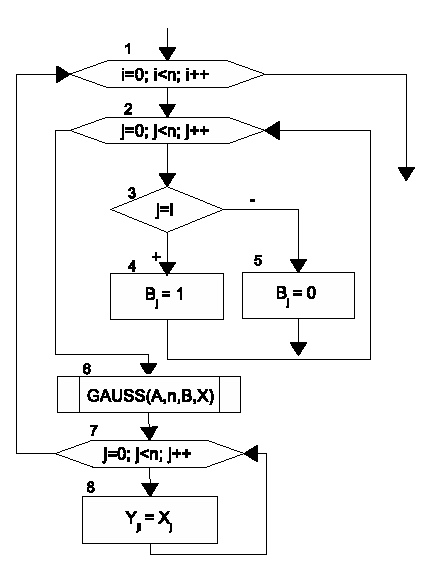
\includegraphics[width=0.8\textwidth]{img/ris_6_16}
\caption{Блок-схема алгоритма вычисления обратной матрицы}
\label{ch06:refDrawing15}
\end{center}
\end{figure}

\prg{Найти определитель квадратной матрицы $A(N,N)$.}{gl06:prg11}

Пусть задана матрица (\ref{gl06:prg1a}), необходимо вычислить ее \emph{определитель}\index{Метод Гаусса!вычисление
определителя}. Для этого матрицу необходимо преобразовать к треугольному виду (\ref{gl06:prg2a}), а затем воспользоваться
свойством, известным из курса линейной алгебры, которое гласит, что определитель треугольной матрицы равен произведению
ее диагональных элементов: $\det A=\prod\limits_{i=0}^{n-1}a_{ii}$.

Преобразование матрицы (\ref{gl06:prg1a}) к виду (\ref{gl06:prg2}) можно осуществить с помощью прямого хода метода Гаусса.
Алгоритм вычисления определителя матрицы, изображённый в виде блок-схемы на рис. \ref{ch06:refDrawing16}, представляет
собой алгоритм прямого хода метода Гаусса, в процессе выполнения которого проводится перестановка строк матрицы. Эта
операция приводит к смене знака определителя. В блок-схеме момент смены знака отражён в блоках 8–9. В блоке 8
определяется, будут ли строки меняться местами, и если ответ утвердительный, то в блоке 9 происходит смена знака
определителя. В блоках 15–16 выполняется непосредственное вычисление определителя путём перемножения диагональных
элементов преобразованной матрицы.

На листинге %\ref{ch06:refDrawing16} 
приведен текст программы решения задачи~\ref{gl06:prg11} с комментариями.
\begin{lstlisting}
#include <iostream>
#include <math.h>
using namespace std;
//`Функция вычисления определителя.`
double determinant(double **matrica_a, int n)
//`Формальные параметры: `matrica_a` --- исходная матрица, `n` --- размер матрицы,` 
//`функция возвращает значение определителя (тип \Sys{double}.)`
{
  int i,j,k,r;
  double c,M,max,s,det=1;
//a` --- копия исходной матрицы.`
  double **a; 
//`Выделение памяти для матрицы `a.
  a=new double *[n];
  for(i=0;i<n;i++)
    a[i]=new double[n];
//`В `a` записываем копию исходной матрицы.`
  for(i=0;i<n;i++)
    for(j=0;j<n;j++)
      a[i][j]=matrica_a[i][j];
//`Прямой ход метода Гаусса.`
  for(k=0;k<n;k++)
  {
    max=fabs(a[k][k]);
    r=k;
    for(i=k+1;i<n;i++)
      if (fabs(a[i][k])>max)
      {
        max=fabs(a[i][k]);
        r=i;
      }
//`Если строки менялись местами, то смена знака определителя.`
    if (r!=k) det=-det;
    for(j=0;j<n;j++)
    {
      c=a[k][j];
      a[k][j]=a[r][j];
      a[r][j]=c;
    }
    for(i=k+1;i<n;i++)
      for(M=a[i][k]/a[k][k],j=k;j<n;j++)
        a[i][j]-=M*a[k][j];
  }
//`Вычисление определителя.`
  for(i=0;i<n;i++)
    det*=a[i][i];
//`Возврат определителя в качестве результата функции.`
  return det;
  for(i=0;i<n;i++)
    delete [] a[i];
  delete [] a;
}
int main()
{
  int result,i,j,N;
  double **a, b; 
  cout<<"N=";
  cin>>N;
  a=new double *[N];
  for(i=0;i<N;i++)
    a[i]=new double[N];
//`Ввод значений исходной матрицы.`
  cout<<"`\Sys{Ввод матрицы}` A"<<endl;
  for(i=0;i<N;i++)
    for(j=0;j<N;j++)
      cin>>a[i][j];
//`Обращение к функции вычисления определителя.`
  cout<<"`\Sys{определитель}`="<<determinant(a,N)<<endl;
}
\end{lstlisting}

\begin{figure}[htb]
\begin{center}
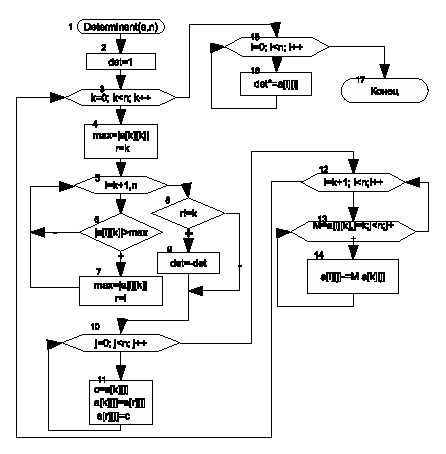
\includegraphics[width=0.8\textwidth]{img/ris_6_17}
\caption{Блок-схема алгоритма вычисления определителя}
\label{ch06:refDrawing16}
\end{center}
\end{figure}

В этой главе читатель познакомился с обработкой статических и динамических матриц в \Sys{C++}, а также с использованием
функций для решения задач обработки динамических матриц. 

\section[Задачи для самостоятельного решения]{Задачи для самостоятельного решения}
\subsection[Основные операции при работе с матрицами]{Основные операции при работе с матрицами}
Разработать программу на языке \Sys{С++} для решения следующей задачи.

\begin{enumerate}
\item В двумерном массиве $A$, состоящем из $n\times n$ целых чисел вычислить: 
\begin{itemize}
\item наименьший элемент;
\item сумму положительных элементов;
\item количество простых чисел, расположенных на диагоналях матрицы
\end{itemize}
Для заданной матрицы $A(n\times n)$ и матрицы того же типа и размерности
$C(n\times n)$ найти значение выражения  $B=2\cdot A+B^T$.

\item В двумерном массиве $C$, состоящем из $n\times n$ целых чисел вычислить:
\begin{itemize}
\item сумму элементов;
\item количество нечетных элементов;
\item минимальное простое число среди элементов, расположенных на главной диагонали.
\end{itemize}

Для заданной матрицы $C(n\times n)$ и матрицы того же типа и размерности
$B(n\times n)$ найти значение выражения  $A=(B-C)\cdot C^T$  

\item В двумерном массиве $B$, состоящем из $m\times m$ целых чисел вычислить: 
\begin{itemize}
\item номер наибольшего элемента;
\item количество отрицательных элементов;
\item среднее геометрическое среди простых чисел, расположенных на побочной диагонали.
\end{itemize}

Для заданной матрицы размерности $B(n\times n)$ найти значение выражения  $A=3\cdot B+B^T$  

\item В двумерном массиве $A$, состоящем из $n\times m$ вещественных чисел вычислить: 
\begin{itemize}
\item сумму элементов;
\item произведение ненулевых элементов;
\item два наибольших значения матрицы.
\end{itemize}

Для заданной матрицы $A(n\times m)$ и матрицы того же типа и размерности
$C(n\times m)$ найти значение выражения  $B=2\cdot A+\frac{1}{3}\cdot C$  

\item В двумерном массиве $B$, состоящем из $n\times m$ вещественных чисел вычислить:
\begin{itemize}
\item произведение элементов;
\item сумму положительных элементов;
\item два наименьших значения среди расположенных выше побочной диагонали.
\end{itemize}

Для заданной матрицы $B(n\times m)$ и матрицы того же типа, но другой размерности  
$C(k\times n)$ найти значение выражения  $A=3\cdot B\cdot C$.

\item В двумерном массиве $A$, состоящем из $n\times n$ целых чисел вычислить: 
\begin{itemize}
\item наименьший элемент;
\item количество четных чисел;
\item сумму положительных элементов, которые представляют собой возрастающую последовательность цифр.
\end{itemize}

Для заданной матрицы $A(n\times n)$ и матрицы того же типа и размерности
$C(n\times n)$ найти значение выражения  $B=A^2-C^T$  

\item В двумерном массиве $C$, состоящем из $n\times n$ целых чисел вычислить:
\begin{itemize}
\item номер наименьшего элемента;
\item сумму квадратов отрицательных элементов;
\item минимальное простое число среди элементов, расположенных в заштрихованной 
части матрицы (рис.~\ref{ch06:refDrawing17}).
\end{itemize}

Для заданной матрицы $C(n\times n)$ и матрицы того же типа и размерности
$B(n\times n)$ найти значение выражения  $A=(B^T+C)^2$  

%%%% рис 6.18 и 6.19 бок о бок
\begin{figure}[H]
\begin{floatrow}
\floatbox{figure}[.45\textwidth][\FBheight][t]
{\caption{}
\label{ch06:refDrawing17}}
{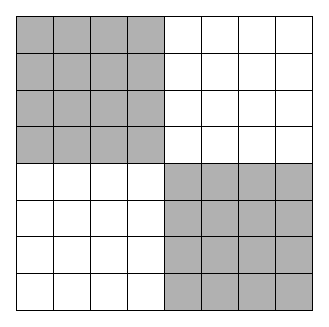
\includegraphics[width=0.45\textwidth,keepaspectratio]{img/ris_6_18}}\hspace*{0.05\textwidth}
%
\floatbox{figure}[.45\textwidth][\FBheight][b]
{\caption{}
\label{ch06:refDrawing18}}
{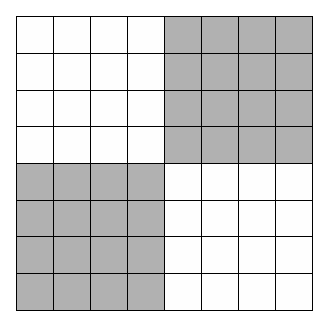
\includegraphics[width=0.45\textwidth,keepaspectratio]{img/ris_6_19}}
\end{floatrow}
\end{figure}
%%%%%%%%%%%%%%%%%%%%%%%%

%{\centering \includegraphics[scale=0.33]{glava6-img019}
%\captionof{figure}[]{}
%\label{ch06:refDrawing17}
%\par}


\item В двумерном массиве $B$, состоящем из $n\times n$ целых чисел вычислить:

\begin{itemize}
\item среднее арифметическое элементов;
\item наименьший четный элемент;
\item количество чисел-палиндромов, расположенных в заштрихованной части матрицы (рис.~\ref{ch06:refDrawing18}).
\end{itemize}
Для заданной матрицы $B(n\times n)$ и матрицы того же типа и размерности
$C(n\times n)$ найти значение выражения  $A=\frac{1}{2}\cdot B+C^2$  

%\centering \includegraphics[scale=0.33]{glava6-img020}
%\captionof{figure}[]{}
%\label{ch06:refDrawing18}
%\par}


\item В двумерном массиве $C$, состоящем из $n\times n$ целых чисел вычислить:

\begin{itemize}
\item среднее геометрическое элементов;
\item наибольший нечетный элемент;
\item количество составных чисел среди элементов, расположенных в заштрихованной 
части матрицы (рис.~\ref{ch06:refDrawing19}).
\end{itemize}
Для заданной матрицы $C(n\times n)$ найти значение выражения  $A=C+C^T$.

\floatsetup[widefloat]{margins=hangleft,labelfont=footnotesize}
\begin{figure}%
\begin{floatrow}[4]
%\captionnamefont{\footnotesize}
\ffigbox[\FBwidth]
{%\captionnamefont{\footnotesize}
\captionsetup{labelfont=footnotesize}\caption{}%
\label{ch06:refDrawing19}}
{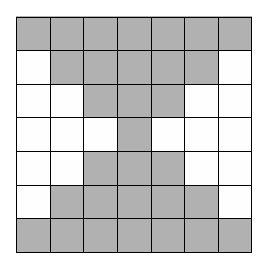
\includegraphics[width=0.225\textwidth,keepaspectratio]{img/ris_6_20}}%\hspace*{0.01\textwidth}

\ffigbox[\FBwidth]
{\caption{}%
\label{ch06:refDrawing20}}
{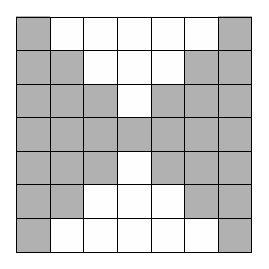
\includegraphics[width=0.225\textwidth,keepaspectratio]{img/ris_6_21}}%\hspace*{0.01\textwidth}

%\ffigbox[\Xhsize/2]
\ffigbox[\FBwidth]%[\FBheight][t]
{\caption{}%
\label{ch06:refDrawing21}}
%{{\setlength\unitlength{\hsize/58}%^^A
{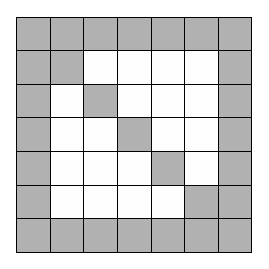
\includegraphics[width=0.225\textwidth,keepaspectratio]{img/ris_6_22}}%\hspace*{0.01\textwidth}
%}}}
%\ffigbox[\Xhsize]
\ffigbox[\FBwidth]%[\FBheight][t]
{\caption{}%
\label{ch06:refDrawing22}}
{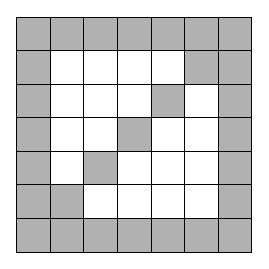
\includegraphics[width=0.225\textwidth,keepaspectratio]{img/ris_6_23}}%}
\end{floatrow}
\end{figure}%


%\centering \includegraphics[scale=0.33]{glava6-img021}
%captionof{figure}[]{}
%label{ch06:refDrawing19}
%par}


\item В двумерном массиве $A$, состоящем из $n\times n$ целых чисел вычислить: 

\begin{itemize}
\item номер наименьшего элемента;
\item среднее арифметическое нечетных чисел;
\item количество положительных элементов, которые представляют собой  убывающую последовательность цифр.
\end{itemize}

Для заданной матрицы $A(n\times n)$ найти значение выражения  $B=\frac{1}{5}\cdot A^2$.
\item В двумерном массиве $B$, состоящем из $n\times n$ вещественных чисел вычислить:
\begin{itemize}
\item среднее арифметическое элементов;
\item элемент наиболее отличающийся от среднего арифметического.
\end{itemize}

Отразить заданную матрицу относительно побочной диагонали.

Для матрицы $B(n\times n)$ и матрицы того же типа и размерности $C(n\times n)$
найти значение выражения  $A=2\cdot B-C^T$.
\item В двумерном массиве $C$, состоящем из $n\times n$ целых чисел вычислить:

\begin{itemize}
\item среднее геометрическое элементов;
\item элемент наименее отличающийся от среднего геометрического;
\item количество положительных элементов с четной суммой цифр, расположенных в заштрихованной 
части матрицы (рис.~\ref{ch06:refDrawing20})
\end{itemize}
Для матрицы $C(n\times n)$ и матрицы того же типа и размерности $B(n\times n)$
найти значение выражения  $A=(B-C)\cdot (B+C)$.

%{\centering \includegraphics[scale=0.33]{glava6-img022}
%\captionof{figure}[]{}
%\label{ch06:refDrawing20}
%\par}

\item В двумерном массиве $A$, состоящем из $n\times n$ целых чисел вычислить:

\begin{itemize}
\item наименьший элемент и его номер;
\item среднее арифметическое положительных четных элементов;
\item произведение простых чисел-палиндромов, расположенных в заштрихованной 
части матрицы (рис.~\ref{ch06:refDrawing21}).
\end{itemize}

Для заданной матрицы $A(n\times n)$ и матрицы того же типа и размерности
$C(n\times n)$ найти значение выражения  $B=A^2-C^2$.

%{\centering \includegraphics[scale=0.33]{glava6-img023}
%\captionof{figure}[]{}
%\label{ch06:refDrawing21}
%\par}


\item В двумерном массиве $C$, состоящем из $n\times n$ целых чисел вычислить:

\begin{itemize}
\item наибольший элемент и его номер;
\item среднее арифметическое элементов, расположенных на диагоналях матрицы.
\end{itemize}

Сформировать новую матрицу $A(n\times n)$, каждый элемент которой будет равен сумме цифр
элемента матрицы $C(n\times n)$. Для матриц $A(n\times n)$ и
$C(n\times n)$ найти значение выражения  $B=(A+C)^2$.
\item В двумерном массиве $B$, состоящем из $m\times m$ целых чисел вычислить: 
\begin{itemize}
\item произведение элементов;
\item номер наибольшего четного элемента;
\item сумму чисел-палиндромов, расположенных вне диагоналей матрицы.
\end{itemize}

Для заданной матрицы размерности $B(n\times n)$ и матрицы того же типа и
размерности $C(n\times n)$ найти значение выражения   $A=C\cdot B-B^T$.
\item В двумерном массиве $A$, состоящем из $n\times n$ целых чисел вычислить:

\begin{itemize}
\item среднее арифметическое элементов;
\item номер наименьшего нечетного элемента, расположенного в заштрихованной части матрицы (рис.~\ref{ch06:refDrawing22}).
\end{itemize}

Сформировать новую матрицу $B(n\times n)$, каждый элемент которой равен значению матрицы
$A(n\times n)$, цифры которого записаны в обратном порядке. Для матриц
$A(n\times n)$ и $B(n\times n)$ найти значение выражения  $B=A+C^2$.

%{\centering \includegraphics[scale=0.33]{glava6-img024}
%\captionof{figure}[]{}
%\label{ch06:refDrawing22}
%\par}


\item В двумерном массиве $A$, состоящем из $n\times m$ целых чисел вычислить: 

\begin{itemize}
\item сумму элементов;
\item количество ненулевых элементов, расположенных по периметру матрицы;
\item среднее геометрическое чисел, состоящих из различных цифр.
\end{itemize}

Для заданной матрицы $A(n\times m)$ и матрицы того же типа и размерности
$C(n\times m)$ найти значение выражения  $B=2\cdot A-3\cdot C$.
\item В двумерном массиве $B$, состоящем из $n\times m$ целых чисел вычислить:

\begin{itemize}
\item произведение элементов;
\item сумму элементов, расположенных вне периметра матрицы;
\item наименьшее число, состоящее из одинаковых цифр.
\end{itemize}

Для заданной матрицы $B(n\times m)$ и матрицы того же типа, но другой размерности
$C(k\times n)$ найти значение выражения  $A=B\cdot C$.
\item В двумерном массиве $A$, состоящем из $n\times n$ целых чисел вычислить:

\begin{itemize}
\item среднее геометрическое элементов;
\item номер наибольшего четного элемента, расположенного в заштрихованной части матрицы (рис.~\ref{ch06:refDrawing23}).
\end{itemize}

Сформировать новую матрицу $B(n\times n)$, каждый элемент которой равен значению матрицы
$A(n\times n)$ в восьмеричной системе счисления. Для матриц $A(n\times n)$ найти
значение выражения  $C=3\cdot A^2$.

%{\centering \includegraphics[scale=0.33]{glava6-img025}
%\captionof{figure}[]{}
%\label{ch06:refDrawing23}
%\par}
\floatsetup[widefloat]{margins=hangleft,labelfont=footnotesize}
\begin{figure}%
\begin{floatrow}[4]
%\captionnamefont{\footnotesize}
\ffigbox[\FBwidth]
{%\captionnamefont{\footnotesize}
\captionsetup{labelfont=footnotesize}\caption{}%
\label{ch06:refDrawing23}}
{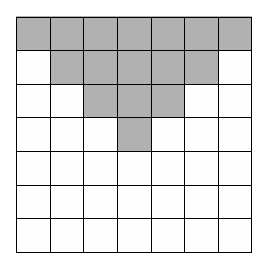
\includegraphics[width=0.225\textwidth,keepaspectratio]{img/ris_6_24}}%\hspace*{0.01\textwidth}

\ffigbox[\FBwidth]
{\caption{}%
\label{ch06:refDrawing24}}
{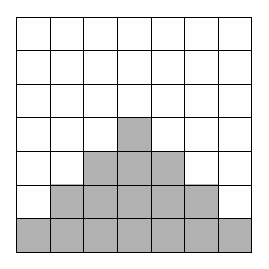
\includegraphics[width=0.225\textwidth,keepaspectratio]{img/ris_6_25}}%\hspace*{0.01\textwidth}

%\ffigbox[\Xhsize/2]
\ffigbox[\FBwidth]%[\FBheight][t]
{\caption{}%
\label{ch06:refDrawing25}}
%{{\setlength\unitlength{\hsize/58}%^^A
{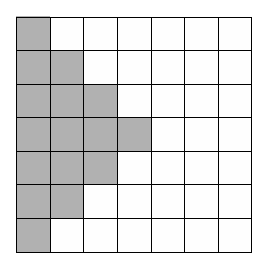
\includegraphics[width=0.225\textwidth,keepaspectratio]{img/ris_6_26}}%\hspace*{0.01\textwidth}
%}}}
%\ffigbox[\Xhsize]
\ffigbox[\FBwidth]%[\FBheight][t]
{\caption{}%
\label{ch06:refDrawing26}}
{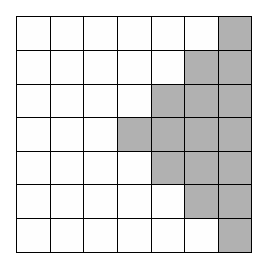
\includegraphics[width=0.225\textwidth,keepaspectratio]{img/ris_6_27}}%}
\end{floatrow}
\end{figure}%



\item В двумерном массиве $B$, состоящем из $n\times n$ целых чисел вычислить:

\begin{itemize}
\item сумму квадратов элементов;
\item количество совершенных чисел, расположенного в заштрихованной части матрицы (рис.~\ref{ch06:refDrawing24}).
\end{itemize}

Сформировать новую матрицу $A(n\times n)$, каждый элемент которой равен количеству делителей
соответствующего значения матрицы $B(n\times n)$. Для матриц $A(n\times n)$ и
$B(n\times n)$ найти значение выражения  $C=B^T-A^2$.

%{\centering \includegraphics[scale=0.33]{glava6-img026}
%\captionof{figure}[]{}
%\label{ch06:refDrawing24}
%\par}


\item В двумерном массиве $A$, состоящем из $n\times n$ целых чисел вычислить:

\begin{itemize}
\item наименьшее абсолютное значение элементов;
\item произведение ненулевых элементов, расположенного в заштрихованной части матрицы (рис.~\ref{ch06:refDrawing25}).
\end{itemize}

Сформировать новую матрицу $B(n\times n)$, каждый элемент которой равен разряду
соответствующего элемента матрицы $A(n\times n)$. Для матриц $A(n\times n)$ найти
значение выражения  $C=B^T\cdot A$.

%{\centering \includegraphics[scale=0.33]{glava6-img027}
%\captionof{figure}[]{}
%\label{ch06:refDrawing25}
%\par}


\item В двумерном массиве $B$, состоящем из $n\times n$ целых чисел вычислить:

\begin{itemize}
\item произведение ненулевых элементов;
\item наибольшее абсолютное значение элементов, расположенного в заштрихованной 
части матрицы (рис.~\ref{ch06:refDrawing26}).
\end{itemize}

Сформировать новую матрицу $C(n\times n)$, каждый элемент которой равен значению матрицы
$B(n\times n)$ в пятеричной системе счисления. Для матриц $B(n\times n)$ найти
значение выражения  $A=B\cdot B^T$.

%{\centering \includegraphics[scale=0.33]{glava6-img028}
%\captionof{figure}[]{}
%\label{ch06:refDrawing26}
%\par}


\item В двумерном массиве $C$, состоящем из $n\times m$ вещественных чисел вычислить:

\begin{itemize}
\item сумму модулей элементов;
\item количество нулевых элементов, расположенных вне периметра матрицы;
\item два наибольших положительных значения.
\end{itemize}

Для заданной матрицы $C(n\times m)$ и матрицы того же типа, но другой размерности
$B(k\times n)$ найти значение выражения  $A=C\cdot B$.

\item В двумерном массиве $B$, состоящем из $n\times m$ вещественных чисел вычислить:

\begin{itemize}
\item сумму квадратов элемента;
\item номер первого нулевого элемента матрицы;
\item два наибольших значения, расположенных вне периметра матрицы;
\end{itemize}

Для заданной матрицы $B(n\times m)$ найти значения выражений  $A=B\cdot B^T$ и 
$C=B^T\cdot B$.
\item В двумерном массиве $A$, состоящем из $n\times n$ вещественных чисел
вычислить:

\begin{itemize}
\item произведение квадратов элемента;
\item номер последнего нулевого элемента матрицы;
\item два наименьших значения, расположенных вне диагоналей матрицы.
\end{itemize}

Из элементов заданной матрицы $A(n\times n)$ сформировать верхнетреугольную матрицу
$V$ и нижнетреугольную матрицу $U$. Проверить равенство  $A=V\cdot U$.
\end{enumerate}

\subsection[Работа со строками и столбцами матрицы]{Работа со строками и столбцами матрицы}
Разработать программу на языке \Sys{С++} для решения следующей задачи.

\begin{enumerate}
\item Задана матрица целых чисел $A(n\times m)$. Сформировать массив
$B(m)$, в который записать среднее арифметическое элементов каждого столбца заданной матрицы.
Вывести номера строк матрицы, в которых находится более двух \emph{простых чисел}.
\item Задана матрица вещественных чисел $B(n\times m)$. Сформировать массив
$A(n)$, в который записать среднее геометрическое положительных элементов каждой строки
заданной матрицы. Определить количество столбцов, упорядоченных по возрастанию.
\item Задана матрица целых чисел $A(n\times n)$. Все \emph{простые числа}, расположенные на
побочной диагонали, заменить \emph{суммой цифр} максимального элемента соответствующей строки матрицы. Сформировать
массив $B(n)$, в который записать произведения элементов нечетных строк заданной матрицы.
\item В матрице целых чисел $X(n\times n)$ поменять местами диагональные элементы,  упорядоченных по
убыванию строк. Сформировать массив $Y(n)$, в который записать суммы элементов четных
столбцов заданной матрицы.
\item Задана матрица целых чисел $A(n\times n)$. Максимальный элемент каждого столбца заменить
\emph{суммой цифр} максимального элемента матрицы. Сформировать массив $B(n)$, в который
записать количество четных элементов в каждой строке заданной матрицы. 
\item Задана матрица целых чисел $B(n\times m)$. Максимальный элемент каждого столбца
заменить \emph{суммой цифр} модуля минимального элемента матрицы. Сформировать массив
$A(n)$, в который записать количество нечетных элементов в каждой строке заданной матрицы.
\item Задана матрица целых чисел $A(n\times n)$. Сформировать массив $B(n)$
из максимальных элементов столбцов заданной матрицы. Вывести номера строк, в которых
числа-палиндромы находятся на диагоналях матрицы. 
\item Задана матрица вещественных чисел $P(n\times m)$. Сформировать массив
$R(k)$ из номеров столбцов матрицы, в которых есть хотя бы один ноль. Найти строку с
максимальной суммой элементов и поменять ее с первой строкой.
\item Задана матрица вещественных чисел $C(k\times m)$. Сформировать вектор
$D(k)$ из средних арифметических положительных значений строк матрицы, и вектор
$G(n)$ из номеров столбцов, которые представляют собой знакочередующийся ряд.
\item В каждом столбце матрицы вещественных чисел $P(k\times m)$ заменить
минимальный элемент суммой положительных элементов этого же столбца. Сформировать вектор
$D(n)$ из номеров строк, представляющих собой знакочередующийся ряд.
\item В матрице целых чисел $A(n\times m)$ обнулить строки, в которых более двух
\emph{простых чисел}. Сформировать вектор $D(m)$ из минимальных значений столбцов матрицы.
\item В матрице вещественных чисел $P(n\times m)$ найти и вывести номера столбцов,
упорядоченных по убыванию элементов. Сформировать вектор $R(n)$ из максимальных значений строк
матрицы.
\item В матрице вещественных чисел $D(n\times m)$ найти и вывести номера строк,
упорядоченных по возрастанию элементов. Сформировать вектор $C(m\times 2)$ из
номеров  минимальных и максимальных значений столбцов матрицы.
\item В матрице вещественных чисел $P(n\times m)$ найти и вывести номера столбцов,
упорядоченных по возрастанию. Сформировать вектор $R(n\times 2)$ из номеров  минимальных и
максимальных значений строк матрицы. 
\item В матрице вещественных чисел $D(n\times m)$ найти и вывести номера строк,
упорядоченных по убыванию. Сформировать вектор $C(m\times 2)$ из максимальных и
минимальных значений столбцов матрицы.
\item В матрице вещественных чисел $X(n\times n)$ найти максимальный и минимальный элементы. Поменять
местами элементы строки с максимальным значением и элементы столбца с минимальным значением.
\item Задана матрица целых чисел $A(n\times n)$. Сформировать массив $B(n)$,
каждый элемент которого равен количеству положительных элементов с чётной суммой цифр в  соответствующей строке
матрицы. В столбцах матрицы поменять местами наибольший и наименьший элементы.
\item Задана матрица целых чисел $A(n\times m)$. Сформировать массив
$B(m)$, каждый элемент которого равен количеству положительных чисел с суммой цифр кратной
трем в  соответствующем столбце матрицы. Найти строку с максимальным произведением элементов.
\item Задана матрица целых чисел $A(n\times n)$. Все \emph{числа-палиндромы},
расположенные на главной диагонали, заменить суммой цифр модуля минимального элемента соответствующего столбца матрицы.
Сформировать вектор $D(n)$ из произведений абсолютных ненулевых значений соответствующих строк
матрицы.
\item Задана матрица целых чисел $A(n\times n)$. Поменять местами элементы на диагоналях в столбцах,
упорядоченных по возрастанию модулей. Сформировать вектор $B(n)$, каждый элемент которого
равен сумме \emph{составных значений} в соответствующей строке матрицы.
\item Задана матрица целых чисел $A(n\times n)$. Минимальный элемент каждой строки заменить суммой
цифр максимального \emph{простого элемента} матрицы. Сформировать вектор $B(n)$,
каждый элемент которого --- среднее геометрическое ненулевых элементов в соответствующем столбце матрицы.
\item Задана матрица целых чисел $A(n\times n)$. Максимальный элемент каждого столбца заменить суммой
цифр минимального \emph{простого элемента} матрицы. Сформировать вектор $B(n)$,
каждый элемент которого равен количеству четных элементов в соответствующей строке матрицы.
\item Задана матрица целых чисел $A(n\times n)$. Обнулить строки, в которых на диагоналях нет
\emph{чисел-палиндромов}. Сформировать вектор $B(n)$, каждый
элемент которого равен количеству нечетных элементов в соответствующем столбце матрицы.
\item Задана матрица вещественных чисел $P(n\times m)$. Найти столбец с минимальным
произведением элементов. Поменять местами элементы этого столбца и элементы последнего столбца. Сформировать вектор
$R(n)$ из сумм квадратов соответствующих строк матрицы.
\item Задана матрица целых чисел $A(n\times m)$. В каждой строке заменить максимальный
элемент \emph{суммой цифр} минимального элемента этой же строки. Сформировать вектор
$B(m\times 2)$, пара элементов которого равна соответственно количеству четных и
нечетных чисел в соответствующем столбце матрицы.
\end{enumerate}

\subsection[Решение задач линейной алгебры]{Решение задач линейной алгебры}
Разработать программу на языке \Sys{С++} для решения следующей задачи.

\begin{enumerate}
\item Задана матрицы $A(n\times n)$ и $B(n\times n)$. Вычислить матрицу 
$C=2(A+B^{-1})-A^T\cdot B$.
\item Задан массив $C(n)$. Сформировать матрицы $A(n\times n)$ и
$B(n\times n)$ по формулам:
 $A_{ij}=C_i\cdot C_j$,  $B_{i,j}=\frac{A_{i,j}}{max(A)}$.

Решить матричное уравнение  $X(A+E)=3B-E$, где $E$ --- единичная матрица.
\item Даны массивы $C(n)$ и $D(n)$. Сформировать матрицы
$A(n\times n)$ и $B(n\times n)$ по формулам:

$A_{ij}=C_i\cdot D_j$,  $B_{i,j}=\frac{A_{i,j}}{min(A)}$.

Решить матричное уравнение  $(2A-E)X=B+E$, где $E$ --- единичная матрица.
\item  Квадратная матрица $A(n\times n)$ называется \emph{ортогональной}, если 
$A^T=A^{-1}$. Определить является ли данная матрица ортогональной:

 $\left(\begin{matrix}1&0.42&0.54&0.66\\0.42&1&0.32&0.44\\0.54&0.32&1&0.22\\0.66&0.44&0.22&1\end{matrix}\right)$.
\item  Для матрицы

  $H=E-\displaystyle\frac{vv^T}{\left|v\right|^2}$, где $E$ --- единичная матрица, 
а $v=\left[\begin{matrix}1\\0\\1\\1\end{matrix}\right]$,

проверить свойство ортогональности:  $H^T=H^{-1}$. 
\item Проверить, образуют ли базис векторы 

$f_1=\left[\begin{matrix}1\\-2\\1\\1\end{matrix}\right], f_2=\left[\begin{matrix}2\\-1\\1\\-1\end{matrix}\right], f_3=\left[\begin{matrix}5\\-2\\-3\\1\end{matrix}\right], f_4=\left[\begin{matrix}1\\-1\\1\\-1\end{matrix}\right]$. 

Если образуют, то найти координаты вектора  $x=[1\ -1\ 3\ -1]^T$  в этом базисе. Для решения задачи необходимо
показать, что определитель матрицы $F$ со столбцами $f_1$, $f_2$, $f_3$, $f_4$  
отличен от нуля, а затем вычислить координаты вектора $x$ в новом базисе по формуле 
$y=F^{-1}\cdot x$.
\item Найти вектор $x$, как решение данной системы уравнений

$\left\{\begin{matrix}
3.75x_1-0.28x_2+0.17x_3=0.75\\
2.11x_1-0.11x_2-0.12x_3=1.11\\
0.22x_1-3.17x_2+1.81x_3=0.05.
\end{matrix}\right.$

Вычислить модуль вектора $x$.
\item  Вычислить скалярное произведение векторов $x$ и $y$. Вектор  $y=|1\ 1\ 2\ -3|$, а вектор
$x$ является решением СЛАУ:

$\left\{\begin{matrix}
5.7x_1-7.8x_2-5.6x_3-8.3x_4=2.7\\
6.6x_1+13.1x_2-6.3x_3+4.3x_4=-5.5\\
14.7x_1-2.8x_2+5.6x_3-12.1x_4=8.6\\
8.5x_1+12.7x_2-23.7x_3+5.7x_4=14.7.
\end{matrix}\right.$
\item Вычислить вектор $X$, решив СЛАУ

$\left\{\begin{matrix}
4.4x_1-2.5x_2+19.2x_3-10.8x_4=4.3\\
5.5x_1-9.3x_2-14.2x_3+13.2x_4=6.8\\
7.1x_1-11.5x_2+5.3x_3-6.7x_4=-1.8\\
14.2x_1+23.4x_2-8.8x_3+5.3x_4=7.2.
\end{matrix}\right.$

Найти  $Y=X\cdot X^T$.
\item Вычислить вектор $X$, решив СЛАУ

$\left\{\begin{matrix}0.34x_1+0.71x_2+0.63x_3=2.08\\0.71x_1-0.65x_2-0.18x_3=0.17\\1.17x_1-2.35x_2+0.75x_3=1.28\end{matrix}\right.$. 

Найти модуль вектора $|2X-3|$.
\item Вычислить угол между векторами $x$ и  $y=|-1\ 5\ -3|$. Вектор $x$ является решением СЛАУ:

$\left\{\begin{matrix}1.24x_1+0.62x_2-0.95x_3=1.43\\2.15x_1-1.18x_2+0.57x_3=2.43\\1.72x_1-0.83x_2+1.57x_3=3.88\end{matrix}\right.$.
\item Решив систему уравнений методом Гаусса:

$\left\{\begin{matrix}8.2x_1-3.2x_2+14.2x_3+14.8x_4=-8.4\\5.6x_1-12x_2+15x_3-6.4x_4=4.5\\5.7x_1+3.6x_2-12.4x_3-2.3x_4=3.3\\6.8x_1+13.2x_2-6.3x_3-8.7x_4=14.3\end{matrix}\right.$.

Вычислить  $H=E-XX^T$.
\item Решить СЛАУ $A^2X=Y^T$, где  $A=\left[\begin{matrix}2&1&5&2\\5&2&2&6\\2&2&1&2\\1&3&3&1\end{matrix}\right]$,
 $Y=|3\ 1\ 2\ 1|$.
\item Решить СЛАУ  $2(A^T)^2X=Y$, где 
$A=\left[\begin{matrix}2&1&5&2\\5&2&2&6\\2&2&1&2\\1&3&3&1\end{matrix}\right]$, 
$Y=\left[\begin{matrix}3\\1\\2\\1\end{matrix}\right]$.
\item Заданы матрицы $A(n\times n)$ и $B(n\times n)$. 

Найти определитель матрицы $C=B^T\cdot A$.
\item  Задан массив $C(n)$. Сформировать матрицы $A(n\times n)$ и
$B(n\times n)$ по формулам:

$A_{ij}=C_i\cdot C_j$,  $B_{ij}=\frac{A_{ij}}{\sum\limits_{i=1}^nA_{ii}}$. Найти
определитель  $|2E-A\cdot B|$.
\item Для матрицы  $I=2P-E$, где $E$ --- единичная матрица, а 
\begin{equation*}
P=\left[\begin{matrix}-26&-18&-27\\21&15&21\\12&8&13\end{matrix}\right]
\end{equation*}
проверить свойство  $I^2=E$. При помощи метода Гаусса решить СЛАУ  $Ix=|1\ 1\ 1|^T$.
\item Квадратная матрица $A(n\times n)$ является \emph{симметричной}, если для нее выполняется
свойство  $A^T=A$. Проверить это свойство для матрицы

$\left(\begin{matrix}
1&0.42&0.54&0.66\\
0.42&1&0.32&0.44\\
0.54&0.32&1&0.22\\
0.66&0.44&0.22&1
\end{matrix}\right)$.

Вычислить  $A^{-1}$. Убедиться, что  $A\cdot A^{-1}=E$.
\item Ортогональная матрица обладает следующими свойствами: 
\begin{itemize}
\item модуль определителя ортогональной матрицы равен 1; 
\item сумма квадратов элементов любого столбца ортогональной матрицы равна 1; 
\item сумма произведений элементов любого столбца ортогональной матрицы на соответствующие элементы другого столбца
равна 0. 
\end{itemize}
Проверить эти свойства для матриц: 

$\left(\begin{matrix}-2&3.01&0.12&-0.11\\2.92&-0.17&0.11&0.22\\0.66&0.52&3.17&2.11\\3.01&0.42&-0.27&-0.15\end{matrix}\right)$
, $\left(\begin{matrix}-2&2.92&0.66&3.01\\2.92&-2&0.11&0.22\\0.66&0.11&-2&2.11\\3.01&0.22&2.11&-2\end{matrix}\right)$.
\item Проверить, образуют ли базис векторы
 
$f_1=\left[\begin{matrix}0.25\\0.333\\0.2\\0.1\end{matrix}\right],f_2=\left[\begin{matrix}0.33\\0.25\\0.167\\0.143\end{matrix}\right],f_3=\left[\begin{matrix}1.25\\-0.667\\2.2\\3.1\end{matrix}\right],f_4=\left[\begin{matrix}-0.667\\1.333\\1.25\\-0.75\end{matrix}\right]$. 

Если образуют, то найти координаты вектора  $x=[1\ 1\ 1\ 1]^T$  в этом базисе. Для решения задачи необходимо показать,
что определитель матрицы $F$ со столбцами  $f_1$, $f_2$, $f_3$, $f_4$ 
отличен от нуля, а затем вычислить координаты вектора $x$ в новом базисе, решив СЛАУ  $F\cdot y=x$. 
\item  Решить СЛАУ:

$\left(\begin{matrix}
0.42&0.26&0.33&-0.22\\
0.74&-0.55&0.28&-0.65\\
0.88&0.42&-0.33&0.75\\
0.92&0.82&-0.62&0.75
\end{matrix}\right)\cdot
X=\left[\begin{matrix}1\\1\\1\\0\end{matrix}\right]$. 

Для матрицы  $C=X\cdot X^T$  проверить условия ортогональности:  $C\cdot C^T=E$  и  $C^T\cdot C=E$.
\item Найти  $\|A\|_1=max\sum\limits_{j=1}^m|a_{ij}|$  и 
$\|A\|_{11}=max\sum\limits_{i=1}^m|a_{ij}|$  для матрицы
 
$\left(\begin{matrix}
0.75&0.18&0.63&-0.32\\
0.92&0.38&-0.14&0.56\\
0.63&-0.42&0.18&0.37\\
-0.65&0.52&0.47&0.27
\end{matrix}\right)^{-1}$.

\item Найти  $\|A\|_{111}=\sqrt{\sum\limits_{i,j}a_{i,j}^2}$  для матрицы 

$\left(\begin{matrix}
-1.09&7.56&3.45&0.78\\
3.33&4.45&-0.21&3.44\\
2.33&-4.45&0.17&2.21\\
4.03&1&3.05&0.11
\end{matrix}\right)^{-1}$.
\item  Решить СЛАУ методом Гаусса
 
$\left\{\begin{matrix}
8.2x_1-3.2x_2+14.2x_3+14.8x_4&=-8.4\\
5.6x_1-12x_2+15x_3-6.4x_4&=4.5\\
5.7x_1+3.6x_2-12.4x_3-2.3x_4&=3.3\\
6.8x_1+13.2x_2-6.3x_3-8.7x_4&=14.3
\end{matrix}\right.$. 

Выполнить проверку  $A\cdot x=b$.
\item Задан массив $H(k)$. Сформировать матрицы $B(k\times k)$ и
$G(k\times k)$ по формулам

 $(B_{ij}=H_i\cdot H_j)$,  $G_{ij}=\displaystyle\frac{B_{ij}}{min(B)}$. 

Решить матричное
уравнение  $(G+E)\cdot X=5B^T-E$, где $E$ --- единичная матрица.
\end{enumerate}

